%********************************************%
%*       Generated from PreTeXt source      *%
%*       on 2024-12-10T16:07:50-05:00       *%
%*   A recent stable commit (2022-07-01):   *%
%* 6c761d3dba23af92cba35001c852aac04ae99a5f *%
%*                                          *%
%*         https://pretextbook.org          *%
%*                                          *%
%********************************************%
\documentclass[twoside, 20pt]{extarticle}
%% Custom Preamble Entries, early (use latex.preamble.early)
%% Always open on odd page
%%   The following adjusts cleardoublepage to remove twosided
%%   check so that we open on odd pages even in one-sided mode
%%   by adding an extra blank page on the preceding even page.
\makeatletter%
\def\cleardoublepage{%
\clearpage\ifodd\c@page\else\thispagestyle{empty}\hbox{}\newpage\if@twocolumn\hbox{}\newpage\fi\fi%
}
\makeatother%
%% Default LaTeX packages
%%   1.  always employed (or nearly so) for some purpose, or
%%   2.  a stylewriter may assume their presence
\usepackage{geometry}
%% Some aspects of the preamble are conditional,
%% the LaTeX engine is one such determinant
\usepackage{ifthen}
%% etoolbox has a variety of modern conveniences
\usepackage{etoolbox}
\usepackage{ifxetex,ifluatex}
%% Raster graphics inclusion
\usepackage{graphicx}
%% Color support, xcolor package
%% Always loaded, for: add/delete text, author tools
%% Here, since tcolorbox loads tikz, and tikz loads xcolor
\PassOptionsToPackage{usenames,dvipsnames,svgnames,table}{xcolor}
\usepackage{xcolor}
%% begin: defined colors, via xcolor package, for styling
%% end: defined colors, via xcolor package, for styling
%% Colored boxes, and much more, though mostly styling
%% skins library provides "enhanced" skin, employing tikzpicture
%% boxes may be configured as "breakable" or "unbreakable"
%% "raster" controls grids of boxes, aka side-by-side
\usepackage{tcolorbox}
\tcbuselibrary{skins}
\tcbuselibrary{breakable}
\tcbuselibrary{raster}
%% We load some "stock" tcolorbox styles that we use a lot
%% Placement here is provisional, there will be some color work also
%% First, black on white, no border, transparent, but no assumption about titles
\tcbset{ bwminimalstyle/.style={enhanced, frame empty, extras broken={
          frame empty}, fonttitle=\bfseries, colback=white, colbacktitle=black!20, coltitle=black, opacityfill=1.0, } }
%% Second, bold title, run-in to text/paragraph/heading
%% Space afterwards will be controlled by environment,
%% independent of constructions of the tcb title
%% Places \blocktitlefont onto many block titles
\tcbset{ runintitlestyle/.style={fonttitle=\blocktitlefont\upshape\bfseries, attach title to upper} }
%% Spacing prior to each exercise, anywhere
\tcbset{ exercisespacingstyle/.style={before skip={1.5ex plus 0.5ex}} }
%% Spacing prior to each block
\tcbset{ blockspacingstyle/.style={before skip={2.0ex plus 0.5ex}} }
%% xparse allows the construction of more robust commands,
%% this is a necessity for isolating styling and behavior
%% The tcolorbox library of the same name loads the base library
\tcbuselibrary{xparse}
%% The tcolorbox library loads TikZ, its calc package is generally useful,
%% and is necessary for some smaller documents that use partial tcolor boxes
%% See:  https://github.com/PreTeXtBook/pretext/issues/1624
\usetikzlibrary{calc}
%% We use some more exotic tcolorbox keys to restore indentation to parboxes
\tcbuselibrary{hooks}
%% Save default paragraph indentation for use later, when adjusting parboxes
\newlength{\normalparindent}
\AtBeginDocument{\setlength{\normalparindent}{\parindent}}
%% Hyperref should be here, but likes to be loaded late
%%
%% Inline math delimiters, \(, \), need to be robust
%% 2016-01-31:  latexrelease.sty  supersedes  fixltx2e.sty
%% If  latexrelease.sty  exists, bugfix is in kernel
%% If not, bugfix is in  fixltx2e.sty
%% See:  https://tug.org/TUGboat/tb36-3/tb114ltnews22.pdf
%% and read "Fewer fragile commands" in distribution's  latexchanges.pdf
\IfFileExists{latexrelease.sty}{}{\usepackage{fixltx2e}}
%% shorter subnumbers in some side-by-side require manipulations
\usepackage{xstring}
%% Footnote counters and part/chapter counters are manipulated
%% April 2018:  chngcntr  commands now integrated into the kernel,
%% but circa 2018/2019 the package would still try to redefine them,
%% so we need to do the work of loading conditionally for old kernels.
%% From version 1.1a,  chngcntr  should detect defintions made by LaTeX kernel.
\ifdefined\counterwithin
\else
    \usepackage{chngcntr}
\fi
%% Text height identically 9 inches, text width varies on point size
%% See Bringhurst 2.1.1 on measure for recommendations
%% 75 characters per line (count spaces, punctuation) is target
%% which is the upper limit of Bringhurst's recommendations
\geometry{letterpaper, inner=1in, outer=0.7in, top=0.4in, bottom=0.7in}
%% Custom Page Layout Adjustments (use publisher page-geometry entry)
%% This LaTeX file may be compiled with pdflatex, xelatex, or lualatex executables
%% LuaTeX is not explicitly supported, but we do accept additions from knowledgeable users
%% The conditional below provides  pdflatex  specific configuration last
%% begin: engine-specific capabilities
\ifthenelse{\boolean{xetex} \or \boolean{luatex}}{%
%% begin: xelatex and lualatex-specific default configuration
\ifxetex\usepackage{xltxtra}\fi
%% realscripts is the only part of xltxtra relevant to lualatex 
\ifluatex\usepackage{realscripts}\fi
%% end:   xelatex and lualatex-specific default configuration
}{
%% begin: pdflatex-specific default configuration
%% We assume a PreTeXt XML source file may have Unicode characters
%% and so we ask LaTeX to parse a UTF-8 encoded file
%% This may work well for accented characters in Western language,
%% but not with Greek, Asian languages, etc.
%% When this is not good enough, switch to the  xelatex  engine
%% where Unicode is better supported (encouraged, even)
\usepackage[utf8]{inputenc}
%% end: pdflatex-specific default configuration
}
%% end:   engine-specific capabilities
%%
%% Fonts.  Conditional on LaTex engine employed.
%% Default Text Font: The Latin Modern fonts are
%% "enhanced versions of the [original TeX] Computer Modern fonts."
%% We use them as the default text font for PreTeXt output.
%% Default Monospace font: Inconsolata (aka zi4)
%% Sponsored by TUG: http://levien.com/type/myfonts/inconsolata.html
%% Loaded for documents with intentional objects requiring monospace
%% See package documentation for excellent instructions
%% fontspec will work universally if we use filename to locate OTF files
%% Loads the "upquote" package as needed, so we don't have to
%% Upright quotes might come from the  textcomp  package, which we also use
%% We employ the shapely \ell to match Google Font version
%% pdflatex: "varl" package option produces shapely \ell
%% pdflatex: "var0" package option produces plain zero (not used)
%% pdflatex: "varqu" package option produces best upright quotes
%% xelatex,lualatex: add OTF StylisticSet 1 for shapely \ell
%% xelatex,lualatex: add OTF StylisticSet 2 for plain zero (not used)
%% xelatex,lualatex: add OTF StylisticSet 3 for upright quotes
%%
%% Fancy Verbatim for consoles, preformatted, code display, literate programming
\usepackage{fancyvrb}
%% Pre-formatted text, a peer of paragraphs
\DefineVerbatimEnvironment{preformatted}{Verbatim}{}
%% Automatic Font Control
%% Portions of a document, are, or may, be affected by defined commands
%% These are perhaps more flexible when using  xelatex  rather than  pdflatex
%% The following definitions are meant to be re-defined in a style, using \renewcommand
%% They are scoped when employed (in a TeX group), and so should not be defined with an argument
\newcommand{\divisionfont}{\relax}
\newcommand{\blocktitlefont}{\relax}
\newcommand{\contentsfont}{\relax}
\newcommand{\pagefont}{\relax}
\newcommand{\tabularfont}{\relax}
\newcommand{\xreffont}{\relax}
\newcommand{\titlepagefont}{\relax}
%%
\ifthenelse{\boolean{xetex} \or \boolean{luatex}}{%
%% begin: font setup and configuration for use with xelatex
%% Generally, xelatex is necessary for non-Western fonts
%% fontspec package provides extensive control of system fonts,
%% meaning *.otf (OpenType), and apparently *.ttf (TrueType)
%% that live *outside* your TeX/MF tree, and are controlled by your *system*
%% (it is possible that a TeX distribution will place fonts in a system location)
%%
%% The fontspec package is the best vehicle for using different fonts in  xelatex
%% So we load it always, no matter what a publisher or style might want
%%
\usepackage{fontspec}
%%
%% begin: xelatex main font ("font-xelatex-main" template)
%% Latin Modern Roman is the default font for xelatex and so is loaded with a TU encoding
%% *in the format* so we can't touch it, only perhaps adjust it later
%% in one of two ways (then known by NFSS names such as "lmr")
%% (1) via NFSS with font family names such as "lmr" and "lmss"
%% (2) via fontspec with commands like \setmainfont{Latin Modern Roman}
%% The latter requires the font to be known at the system-level by its font name,
%% but will give access to OTF font features through optional arguments
%% https://tex.stackexchange.com/questions/470008/
%% where-and-how-does-fontspec-sty-specify-the-default-font-latin-modern-roman
%% http://tex.stackexchange.com/questions/115321
%% /how-to-optimize-latin-modern-font-with-xelatex
%%
%% end:   xelatex main font ("font-xelatex-main" template)
%% begin: xelatex mono font ("font-xelatex-mono" template)
%% (conditional on non-trivial uses being present in source)
\IfFontExistsTF{Inconsolatazi4-Regular.otf}{}{\GenericError{}{The font "Inconsolatazi4-Regular.otf" requested by PreTeXt output is not available.  Either a file cannot be located in default locations via a filename, or a font is not known by its name as part of your system.}{Consult the PreTeXt Guide for help with LaTeX fonts.}{}}
\IfFontExistsTF{Inconsolatazi4-Bold.otf}{}{\GenericError{}{The font "Inconsolatazi4-Bold.otf" requested by PreTeXt output is not available.  Either a file cannot be located in default locations via a filename, or a font is not known by its name as part of your system.}{Consult the PreTeXt Guide for help with LaTeX fonts.}{}}
\usepackage{zi4}
\setmonofont[BoldFont=Inconsolatazi4-Bold.otf,StylisticSet={1,3}]{Inconsolatazi4-Regular.otf}
%% end:   xelatex mono font ("font-xelatex-mono" template)
%% begin: xelatex font adjustments ("font-xelatex-style" template)
%% end:   xelatex font adjustments ("font-xelatex-style" template)
%%
%% Extensive support for other languages
\usepackage{polyglossia}
%% Set main/default language based on pretext/@xml:lang value
%% document language code is "es-ES", Spanish
\setmainlanguage{spanish}
%% Enable secondary languages based on discovery of @xml:lang values
%% Enable fonts/scripts based on discovery of @xml:lang values
%% Western languages should be ably covered by Latin Modern Roman
%% end:   font setup and configuration for use with xelatex
}{%
%% begin: font setup and configuration for use with pdflatex
%% begin: pdflatex main font ("font-pdflatex-main" template)
\usepackage{lmodern}
\usepackage[T1]{fontenc}
%% end:   pdflatex main font ("font-pdflatex-main" template)
%% begin: pdflatex mono font ("font-pdflatex-mono" template)
%% (conditional on non-trivial uses being present in source)
\usepackage[varqu,varl]{inconsolata}
%% end:   pdflatex mono font ("font-pdflatex-mono" template)
%% begin: pdflatex font adjustments ("font-pdflatex-style" template)
%% end:   pdflatex font adjustments ("font-pdflatex-style" template)
%% end:   font setup and configuration for use with pdflatex
}
%% Micromanage spacing, etc.  The named "microtype-options"
%% template may be employed to fine-tune package behavior
\usepackage{microtype}
%% Symbols, align environment, commutative diagrams, bracket-matrix
\usepackage{amsmath}
\usepackage{amscd}
\usepackage{amssymb}
%% allow page breaks within display mathematics anywhere
%% level 4 is maximally permissive
%% this is exactly the opposite of AMSmath package philosophy
%% there are per-display, and per-equation options to control this
%% split, aligned, gathered, and alignedat are not affected
\allowdisplaybreaks[4]
%% allow more columns to a matrix
%% can make this even bigger by overriding with  latex.preamble.late  processing option
\setcounter{MaxMatrixCols}{30}
%%
%%
%% Division Titles, and Page Headers/Footers
%% titlesec package, loading "titleps" package cooperatively
%% See code comments about the necessity and purpose of "explicit" option.
%% The "newparttoc" option causes a consistent entry for parts in the ToC 
%% file, but it is only effective if there is a \titleformat for \part.
%% "pagestyles" loads the  titleps  package cooperatively.
\usepackage[explicit, newparttoc, pagestyles]{titlesec}
%% The companion titletoc package for the ToC.
\usepackage{titletoc}
%% begin: customizations of page styles via the modal "titleps-style" template
%% Designed to use commands from the LaTeX "titleps" package
\pagestyle{plain}
%% end: customizations of page styles via the modal "titleps-style" template
%%
%% Create globally-available macros to be provided for style writers
%% These are redefined for each occurence of each division
%
% Number subsections ignoring sections
\renewcommand{\thesubsection}{\arabic{subsection}}
\makeatletter
\@removefromreset{subsection}{section}
\makeatother
%
%
\newcommand{\divisionnameptx}{\relax}%
\newcommand{\titleptx}{\relax}%
\newcommand{\subtitleptx}{\relax}%
\newcommand{\shortitleptx}{\relax}%
\newcommand{\authorsptx}{\relax}%
\newcommand{\epigraphptx}{\relax}%
%% Create environments for possible occurences of each division
%% Environment for a PTX "section" at the level of a LaTeX "section"
\NewDocumentEnvironment{sectionptx}{mmmmmmm}
{%
\renewcommand{\divisionnameptx}{#1}%
\renewcommand{\titleptx}{#2}%
\renewcommand{\subtitleptx}{#3}%
\renewcommand{\shortitleptx}{#4}%
\renewcommand{\authorsptx}{#5}%
\renewcommand{\epigraphptx}{#6}%
% \section{}%[{#4}]{#2}%
% \label{#7}%
\vspace*{-\topskip}%
\relax
% \clearpage
}{}%
%% Environment for a PTX "subsection" at the level of a LaTeX "subsection"
\NewDocumentEnvironment{subsectionptx}{mmmmmmm}
{%
\renewcommand{\divisionnameptx}{#1}%
\renewcommand{\titleptx}{#2}%
\renewcommand{\subtitleptx}{#3}%
\renewcommand{\shortitleptx}{#4}%
\renewcommand{\authorsptx}{#5}%
\renewcommand{\epigraphptx}{#6}%
% \vspace{-1.5cm}
\vspace*{-\topskip}%
\subsection{}%[{#4}]{#2}%
% \vspace{-0.7cm}
\label{#7}%
}{}%
%% Environment for a PTX "reading-questions" at the level of a LaTeX "subsubsection"
\NewDocumentEnvironment{reading-questions-subsubsection}{mmmmmmm}
{%
\renewcommand{\divisionnameptx}{#1}%
\renewcommand{\titleptx}{#2}%
\renewcommand{\subtitleptx}{#3}%
\renewcommand{\shortitleptx}{#4}%
\renewcommand{\authorsptx}{#5}%
\renewcommand{\epigraphptx}{#6}%
% \clearpage
\vspace*{-\topskip}%
\subsubsection[{#4}]{Lección~\thesubsection~-~#2}%
\vspace{-0.7cm}
\label{#7}%
}{}%
%% Environment for a PTX "reading-questions" at the level of a LaTeX "subsubsection"
\NewDocumentEnvironment{reading-questions-subsubsection-numberless}{mmmmmmm}
{%
\renewcommand{\divisionnameptx}{#1}%
\renewcommand{\titleptx}{#2}%
\renewcommand{\subtitleptx}{#3}%
\renewcommand{\shortitleptx}{#4}%
\renewcommand{\authorsptx}{#5}%
\renewcommand{\epigraphptx}{#6}%
% \clearpage
\vspace*{-\topskip}%
\subsubsection*{Lección~\thesubsection~-~#2}%
\vspace{-0.7cm}
\addcontentsline{toc}{subsubsection}{#4}
\label{#7}%
}{}%
%% Environment for a PTX "subsubsection" at the level of a LaTeX "subsubsection"
\NewDocumentEnvironment{subsubsectionptx}{mmmmmmm}
{%
\renewcommand{\divisionnameptx}{#1}%
\renewcommand{\titleptx}{#2}%
\renewcommand{\subtitleptx}{#3}%
\renewcommand{\shortitleptx}{#4}%
\renewcommand{\authorsptx}{#5}%
\renewcommand{\epigraphptx}{#6}%
% \clearpage
% \vspace{-1.0cm}
\vspace*{-1.5\topskip}%
\subsubsection[{#4}]{Lección~\thesubsection~-~#2}%
% \vspace{-0.7cm}
\label{#7}%
}{}%
%% Environment for a PTX "exercises" at the level of a LaTeX "subsection"
\NewDocumentEnvironment{exercises-subsection}{mmmmmmm}
{%
\renewcommand{\divisionnameptx}{#1}%
\renewcommand{\titleptx}{#2}%
\renewcommand{\subtitleptx}{#3}%
\renewcommand{\shortitleptx}{#4}%
\renewcommand{\authorsptx}{#5}%
\renewcommand{\epigraphptx}{#6}%
\clearpage
\subsection*{#2}%
\label{#7}%
}{}%
%% Environment for a PTX "exercises" at the level of a LaTeX "subsection"
\NewDocumentEnvironment{exercises-subsection-numberless}{mmmmmmm}
{%
\renewcommand{\divisionnameptx}{#1}%
\renewcommand{\titleptx}{#2}%
\renewcommand{\subtitleptx}{#3}%
\renewcommand{\shortitleptx}{#4}%
\renewcommand{\authorsptx}{#5}%
\renewcommand{\epigraphptx}{#6}%
% \subsection*{#2}%
\subsection[{#4}]{Lección~\thesubsection - #2}
\addcontentsline{toc}{subsection}{Lección~\thesubsection - #4}
\label{#7}%
}{}%
%% Environment for a PTX "references" at the level of a LaTeX "subsection"
\NewDocumentEnvironment{references-subsection}{mmmmmmm}
{%
\renewcommand{\divisionnameptx}{#1}%
\renewcommand{\titleptx}{#2}%
\renewcommand{\subtitleptx}{#3}%
\renewcommand{\shortitleptx}{#4}%
\renewcommand{\authorsptx}{#5}%
\renewcommand{\epigraphptx}{#6}%
\subsection[{#4}]{Lección~\thesubsection - #2}%
\label{#7}%
}{}%
%% Environment for a PTX "references" at the level of a LaTeX "subsection"
\NewDocumentEnvironment{references-subsection-numberless}{mmmmmmm}
{%
\renewcommand{\divisionnameptx}{#1}%
\renewcommand{\titleptx}{#2}%
\renewcommand{\subtitleptx}{#3}%
\renewcommand{\shortitleptx}{#4}%
\renewcommand{\authorsptx}{#5}%
\renewcommand{\epigraphptx}{#6}%
\subsection*{#2}%
\addcontentsline{toc}{subsection}{Lección~\thesubsection - #4}
\label{#7}%
}{}%
%% Environment for a PTX "references" at the level of a LaTeX "section"
\NewDocumentEnvironment{references-section}{mmmmmmm}
{%
\renewcommand{\divisionnameptx}{#1}%
\renewcommand{\titleptx}{#2}%
\renewcommand{\subtitleptx}{#3}%
\renewcommand{\shortitleptx}{#4}%
\renewcommand{\authorsptx}{#5}%
\renewcommand{\epigraphptx}{#6}%
\section[{#4}]{#2}%
\label{#7}%
}{}%
%% Environment for a PTX "references" at the level of a LaTeX "section"
\NewDocumentEnvironment{references-section-numberless}{mmmmmmm}
{%
\renewcommand{\divisionnameptx}{#1}%
\renewcommand{\titleptx}{#2}%
\renewcommand{\subtitleptx}{#3}%
\renewcommand{\shortitleptx}{#4}%
\renewcommand{\authorsptx}{#5}%
\renewcommand{\epigraphptx}{#6}%
\section*{#2}%
\addcontentsline{toc}{section}{#4}
\label{#7}%
}{}%
%%
%% Styles for six traditional LaTeX divisions
\titleformat{\part}[display]
{\divisionfont\Huge\bfseries\centering}{\divisionnameptx\space\thepart}{30pt}{\Huge#1}
[{\Large\centering\authorsptx}]
\titleformat{\chapter}[display]
{\divisionfont\huge\bfseries}{\divisionnameptx\space\thechapter}{20pt}{\Huge#1}
[{\Large\authorsptx}]
\titleformat{name=\chapter,numberless}[display]
{\divisionfont\huge\bfseries}{}{0pt}{#1}
[{\Large\authorsptx}]
\titlespacing*{\chapter}{0pt}{50pt}{40pt}
\titleformat{\section}[hang]
{\divisionfont\Large\bfseries}{}{1ex}{#1}
[{\large\authorsptx}]
\titleformat{name=\section,numberless}[block]
{\divisionfont\Large\bfseries}{}{0pt}{#1}
[{\large\authorsptx}]
\titlespacing*{\section}{0pt}{0ex plus 0ex minus 0ex}{-1ex plus 0ex}
\titleformat{\subsection}[hang]
{\divisionfont\large\bfseries}{}{1ex}{#1}
[{\normalsize\authorsptx}]
\titleformat{name=\subsection,numberless}[block]
{\divisionfont\large\bfseries}{}{0pt}{#1}
[{\normalsize\authorsptx}]
\titlespacing*{\subsection}{0pt}{0ex plus 0ex minus 0.5ex}{0ex plus 0ex minus 0.5ex}
\titleformat{\subsubsection}[hang]
{\divisionfont\normalsize\bfseries}{\thesubsubsection}{1em}{#1}
[{\small\authorsptx}]
\titleformat{name=\subsubsection,numberless}[block]
{\divisionfont\normalsize\bfseries}{}{0pt}{#1}
[{\normalsize\authorsptx}]
\titlespacing*{\subsubsection}{0pt}{2ex plus 2ex minus 0ex}{-1ex plus 0ex}
\titleformat{\paragraph}[hang]
{\divisionfont\normalsize\bfseries}{\theparagraph}{1em}{#1}
[{\small\authorsptx}]
\titleformat{name=\paragraph,numberless}[block]
{\divisionfont\normalsize\bfseries}{}{0pt}{#1}
[{\normalsize\authorsptx}]
\titlespacing*{\paragraph}{0pt}{1.25ex plus 1ex minus .2ex}{1.5em}
%%
%% Styles for five traditional LaTeX divisions
\titlecontents{part}%
[0pt]{\contentsmargin{0em}\addvspace{1pc}\contentsfont\bfseries}%
{\Large\thecontentslabel\enspace}{\Large}%
{}%
[\addvspace{.5pc}]%
\titlecontents{chapter}%
[0pt]{\contentsmargin{0em}\addvspace{1pc}\contentsfont\bfseries}%
{\large\thecontentslabel\enspace}{\large}%
{\hfill\bfseries\thecontentspage}%
[\addvspace{.5pc}]%
\dottedcontents{section}[3.8em]{\contentsfont}{2.3em}{1pc}%
\dottedcontents{subsection}[6.1em]{\contentsfont}{3.2em}{1pc}%
\dottedcontents{subsubsection}[9.3em]{\contentsfont}{4.3em}{1pc}%
%%
%% Begin: Semantic Macros
%% To preserve meaning in a LaTeX file
%%
%% \mono macro for content of "c", "cd", "tag", etc elements
%% Also used automatically in other constructions
%% Simply an alias for \texttt
%% Always defined, even if there is no need, or if a specific tt font is not loaded
\newcommand{\mono}[1]{\texttt{#1}}
%%
%% Following semantic macros are only defined here if their
%% use is required only in this specific document
%%
%% Used for warnings, typically bold and italic
\newcommand{\alert}[1]{\textbf{\textit{#1}}}
%% Used for fillin answer blank in text
%% Relies on calc package, loaded via tcolorbox
%% Argument is intended number of characters of blank
%% Length may compress for output to fit in one line
\newlength{\fillinmaxwidth}
\newlength{\fillincontract}
\newlength{\fillinheight}
\newcommand{\fillintext}[1]{%
\setlength{\fillinmaxwidth}{#1em*\real{0.5}}%
\setlength{\fillincontract}{#1em*\real{0.5}*\real{0.2}}%
\setlength{\fillinheight}{\heightof{\strut}+1.2pt}%
\strut\nobreak\leaders\vbox{\hrule width 0.3pt height 0.3pt \vskip -1.2pt}\hskip 1\fillinmaxwidth minus \fillincontract\nobreak\strut%
}
%% End: Semantic Macros
%% Divisional exercises (and worksheet) as LaTeX environments
%% Third argument is option for extra workspace in worksheets
%% Hanging indent occupies a 5ex width slot prior to left margin
%% Experimentally this seems just barely sufficient for a bold "888."
%% Division exercises, not in exercise group
\tcbset{ divisionexercisestyle/.style={bwminimalstyle, runintitlestyle, exercisespacingstyle, left=2.3cm, breakable, before upper app={\setlength{\parskip}{\medskipamount}} } }
\newtcolorbox{divisionexercise}[4]{divisionexercisestyle, before title={\hspace{-5ex}\makebox[5ex][l]{#1.}}, title={\notblank{#2}{#2\space}{}}, phantom={\label{#4}\hypertarget{#4}{}}, after={}}
%% "tcolorbox" environment for a single image, occupying entire \linewidth
%% arguments are left-margin, width, right-margin, as multiples of
%% \linewidth, and are guaranteed to be positive and sum to 1.0
\tcbset{ imagestyle/.style={bwminimalstyle, blankest} }
\NewTColorBox{tcbimage}{mmm}{imagestyle}
%% Wrapper environment for tcbimage environment with a fourth argument
%% Fourth argument, if nonempty, is a vertical space adjustment
%% and implies image will be preceded by \leavevmode\nopagebreak
%% Intended use is for alignment with a list marker
\NewDocumentEnvironment{image}{mmmm}{\notblank{#4}{\leavevmode\nopagebreak\vspace{#4}}{~\par}\begin{tcbimage}{#1}{#2}{#3}}{\end{tcbimage}%
}%% For improved tables
\usepackage{array}
%% Some extra height on each row is desirable, especially with horizontal rules
%% Increment determined experimentally
\setlength{\extrarowheight}{0.2ex}
%% Define variable thickness horizontal rules, full and partial
%% Thicknesses are 0.03, 0.05, 0.08 in the  booktabs  package
\newcommand{\hrulethin}  {\noalign{\hrule height 0.04em}}
\newcommand{\hrulemedium}{\noalign{\hrule height 0.07em}}
\newcommand{\hrulethick} {\noalign{\hrule height 0.11em}}
%% We preserve a copy of the \setlength package before other
%% packages (extpfeil) get a chance to load packages that redefine it
\let\oldsetlength\setlength
\newlength{\Oldarrayrulewidth}
\newcommand{\crulethin}[1]%
{\noalign{\global\oldsetlength{\Oldarrayrulewidth}{\arrayrulewidth}}%
\noalign{\global\oldsetlength{\arrayrulewidth}{0.04em}}\cline{#1}%
\noalign{\global\oldsetlength{\arrayrulewidth}{\Oldarrayrulewidth}}}%
\newcommand{\crulemedium}[1]%
{\noalign{\global\oldsetlength{\Oldarrayrulewidth}{\arrayrulewidth}}%
\noalign{\global\oldsetlength{\arrayrulewidth}{0.07em}}\cline{#1}%
\noalign{\global\oldsetlength{\arrayrulewidth}{\Oldarrayrulewidth}}}
\newcommand{\crulethick}[1]%
{\noalign{\global\oldsetlength{\Oldarrayrulewidth}{\arrayrulewidth}}%
\noalign{\global\oldsetlength{\arrayrulewidth}{0.11em}}\cline{#1}%
\noalign{\global\oldsetlength{\arrayrulewidth}{\Oldarrayrulewidth}}}
%% Single letter column specifiers defined via array package
\newcolumntype{A}{!{\vrule width 0.04em}}
\newcolumntype{B}{!{\vrule width 0.07em}}
\newcolumntype{C}{!{\vrule width 0.11em}}
%% tcolorbox to place tabular outside of a sidebyside
\tcbset{ tabularboxstyle/.style={bwminimalstyle,} }
\newtcolorbox{tabularbox}[3]{tabularboxstyle, left skip=#1\linewidth, width=#2\linewidth,}
%% Footnote Numbering
%% Specified by numbering.footnotes.level
%% Global numbering, since numbering.footnotes.level = 0
%% Multiple column, column-major lists
\usepackage{multicol}
%% More flexible list management, esp. for references
%% But also for specifying labels (i.e. custom order) on nested lists
\usepackage{enumitem}
\setlist{nosep, topsep=0pt, partopsep=0.3ex, parsep=1ex}
%% Lists of references in their own section, maximum depth 1
\newlist{referencelist}{description}{4}
\setlist[referencelist]{leftmargin=!,labelwidth=!,labelsep=0ex,itemsep=1.0ex,topsep=1.0ex,partopsep=0pt,parsep=0pt}
%% Description lists as tcolorbox sidebyside
%% "dli" short for "description list item"
\newlength{\dlititlewidth}
\newlength{\dlimaxnarrowtitle}\setlength{\dlimaxnarrowtitle}{11ex}
\newlength{\dlimaxmediumtitle}\setlength{\dlimaxmediumtitle}{18ex}
\tcbset{ dlistyle/.style={sidebyside, sidebyside align=top seam, lower separated=false, bwminimalstyle, bottomtitle=0.75ex, after skip=1.5ex, boxsep=0pt, left=0pt, right=0pt, top=0pt, bottom=0pt} }
\tcbset{ dlinarrowstyle/.style={dlistyle, lefthand width=\dlimaxnarrowtitle, sidebyside gap=1ex, halign=flush left, righttitle=10ex} }
\tcbset{ dlimediumstyle/.style={dlistyle, lefthand width=\dlimaxmediumtitle, sidebyside gap=4ex, halign=flush right} }
\NewDocumentEnvironment{descriptionlist}{}{\par\vspace*{1.5ex}}{\par\vspace*{1.5ex}}%
%% begin enviroment has an if/then to open the tcolorbox
\NewDocumentEnvironment{dlinarrow}{mm}{%
\settowidth{\dlititlewidth}{{\textbf{#1}}}%
\ifthenelse{\dlititlewidth > \dlimaxnarrowtitle}%
{\begin{tcolorbox}[title={\textbf{#1}}, phantom={\hypertarget{#2}{}}, dlinarrowstyle]\tcblower}%
{\begin{tcolorbox}[dlinarrowstyle, phantom={\hypertarget{#2}{}}]\textbf{#1}\tcblower}%
}%
{\end{tcolorbox}}%
%% medium option is simpler
\NewDocumentEnvironment{dlimedium}{mm}%
{\begin{tcolorbox}[dlimediumstyle, phantom={\hypertarget{#2}{}}]\textbf{#1}\tcblower}%
{\end{tcolorbox}}%
%% hyperref driver does not need to be specified, it will be detected
%% Footnote marks in tcolorbox have broken linking under
%% hyperref, so it is necessary to turn off all linking
%% It *must* be given as a package option, not with \hypersetup
\usepackage[hyperfootnotes=false]{hyperref}
%% configure hyperref's  \href{}{}  and  \nolinkurl  to match listings' inline verbatim
\renewcommand\UrlFont{\small\ttfamily}
%% For a print PDF, no surrounding boxes, so simply textcolor (but still active to preserve spacing)
\hypersetup{hidelinks=true}
%% Less-clever names for hyperlinks are more reliable, *especially* for structural parts
%% See comments in the code to learn more about the importance of this setting
\hypersetup{hypertexnames=false}
%%The  hypertexnames  setting then confuses the hyperlinking from the index
%%This patch resolves the incorrect links, see code for StackExchange post.
\makeatletter
\patchcmd\Hy@EveryPageBoxHook{\Hy@EveryPageAnchor}{\Hy@hypertexnamestrue\Hy@EveryPageAnchor}{}{\fail}
\makeatother
\hypersetup{pdftitle={Matemáticas Ilustrativas}}
%% If you manually remove hyperref, leave in this next command
%% This will allow LaTeX compilation, employing this no-op command
\providecommand\phantomsection{}
%% Division Numbering: Chapters, Sections, Subsections, etc
%% Division numbers may be turned off at some level ("depth")
%% A section *always* has depth 1, contrary to us counting from the document root
%% The latex default is 3.  If a larger number is present here, then
%% removing this command may make some cross-references ambiguous
%% The precursor variable $numbering-maxlevel is checked for consistency in the common XSL file
\setcounter{secnumdepth}{2}
%%
%% AMS "proof" environment is no longer used, but we leave previously
%% implemented \qedhere in place, should the LaTeX be recycled
\newcommand{\qedhere}{\relax}
%%
%% A faux tcolorbox whose only purpose is to provide common numbering
%% facilities for most blocks (possibly not projects, 2D displays)
%% Controlled by  numbering.theorems.level  processing parameter
\newtcolorbox[auto counter]{block}{}
%%
%% This document is set to number PROJECT-LIKE on a separate numbering scheme
%% So, a faux tcolorbox whose only purpose is to provide this numbering
%% Controlled by  numbering.projects.level  processing parameter
\newtcolorbox[auto counter]{project-distinct}{}
%% A faux tcolorbox whose only purpose is to provide common numbering
%% facilities for 2D displays which are subnumbered as part of a "sidebyside"
\makeatletter
\newtcolorbox[auto counter, number within=tcb@cnt@block, number freestyle={\noexpand\thetcb@cnt@block(\noexpand\alph{\tcbcounter})}]{subdisplay}{}
\makeatother
%%
%% tcolorbox, with styles, for PROJECT-LIKE
%%
%% project: fairly simple numbered block/structure
\tcbset{ projectstyle/.style={bwminimalstyle, blockspacingstyle, before title={\vspace{0.3em}\strut}, after title={\strut\vspace{0.15em}}, before upper app={\setlength{\parskip}{\medskipamount}}, } }
\newtcolorbox[use counter from=project-distinct]{project}[3]{title={#2}, phantomlabel={#3}, breakable, after={\par}, projectstyle, }
%% activity: fairly simple numbered block/structure
\tcbset{ activitystyle/.style={bwminimalstyle, blockspacingstyle, before title={\vspace{0.3em}}, after title={\strut\vspace{0.15em}}, before upper app={\setlength{\parskip}{\medskipamount}}}, }
\newtcolorbox[use counter from=project-distinct]{activity}[3]{title={#2}, phantomlabel={#3}, breakable, after={\par}, activitystyle, }
%% exploration: fairly simple numbered block/structure
\tcbset{ explorationstyle/.style={bwminimalstyle, runintitlestyle, blockspacingstyle, after title={\space}, before upper app={\setlength{\parskip}{\medskipamount}}, } }
\newtcolorbox[use counter from=project-distinct]{exploration}[3]{title={{#1~\thetcbcounter\notblank{#2}{\space\space#2}{}}}, phantomlabel={#3}, breakable, after={\par}, explorationstyle, }
%%
%% xparse environments for introductions and conclusions of divisions
%%
%% paragraphs: the terminal, pseudo-division
%% We use the lowest LaTeX traditional division
\titleformat{\subparagraph}[runin]{\normalfont\normalsize\bfseries}{\thesubparagraph}{1em}{#1}
\titlespacing*{\subparagraph}{0pt}{3.25ex plus 1ex minus .2ex}{1em}
\NewDocumentEnvironment{paragraphs}{mm}
{\subparagraph*{#1}\hypertarget{#2}{}}{}
%% introduction: in a structured division
\NewDocumentEnvironment{introduction}{m}
{\notblank{#1}{\noindent\textbf{#1}\space}{}}{\par\medskip}
%% Graphics Preamble Entries
\usepackage{tikz, pgfplots}
\usetikzlibrary{positioning,matrix,arrows}
\usetikzlibrary{shapes,decorations,shadows,fadings,patterns}
\usetikzlibrary{decorations.markings}
%% If tikz has been loaded, replace ampersand with \amp macro
%% tcolorbox styles for sidebyside layout
\tcbset{ sbsstyle/.style={raster before skip=0.3ex, raster equal height=rows, raster force size=false, } }
\tcbset{ sbspanelstyle/.style={bwminimalstyle, fonttitle=\blocktitlefont, } }
%% Enviroments for side-by-side and components
%% Necessary to use \NewTColorBox for boxes of the panels
%% "newfloat" environment to squash page-breaks within a single sidebyside
%% "xparse" environment for entire sidebyside
\NewDocumentEnvironment{sidebyside}{mmmm}
  {\begin{tcbraster}
    [sbsstyle,raster columns=#1,
    raster left skip=#2\linewidth,raster right skip=#3\linewidth,raster column skip=#4\linewidth, ]}
  {\end{tcbraster}}
%% "tcolorbox" environment for a panel of sidebyside
\NewTColorBox{sbspanel}{mO{top}}{sbspanelstyle,width=#1\linewidth,valign=#2, }
%% Custom Preamble Entries, late (use latex.preamble.late)
%% extpfeil package for certain extensible arrows,
%% as also provided by MathJax extension of the same name
%% NB: this package loads mtools, which loads calc, which redefines
%%     \setlength, so it can be removed if it seems to be in the 
%%     way and your math does not use:
%%     
%%     \xtwoheadrightarrow, \xtwoheadleftarrow, \xmapsto, \xlongequal, \xtofrom
%%     
%%     we have had to be extra careful with variable thickness
%%     lines in tables, and so also load this package late
\usepackage{extpfeil}
%% Begin: Author-provided macros
%% (From  docinfo/macros  element)
%% Plus three from PTX for XML characters
\newcommand{\boldcdot}{\boldsymbol{\cdot}}
\newcommand{\unit}[1]{\,\text{#1}}
\newcommand{\lt}{<}
\newcommand{\gt}{>}
\newcommand{\amp}{&}
\usepackage[export]{adjustbox}% 'export' allows adjustbox keys in \includegraphics
% \renewcommand{\familydefault}{\sfdefault}
\usepackage[sfdefault]{roboto} 
\usepackage{sansmath}
\sansmath % Apply sansmath globally to all math environments
% \usepackage{microtype}
% stop hyphenation
\setlength{\emergencystretch}{3em}
\tolerance=1000
\hbadness=1000
\usepackage[none]{hyphenat} % Disable hyphenation
\hyphenpenalty=10000
\exhyphenpenalty=10000
% estilo de párrafos
\setlength{\parindent}{0pt}    % No indentation for new paragraphs
\setlength{\parskip}{1ex}     % Small space between paragraphs 
% Quitar justificación (lineas igual de anchas)
\usepackage[document]{ragged2e}
% headers y footers
\usepackage{fancyhdr}
\pagestyle{fancy}
\fancyfoot[C]{} %Remove default Latex numbering
\fancyhead[C]{\begin{tikzpicture}[remember picture,overlay] \node[yshift=-0.5cm] at (current page.north west) {\begin{tikzpicture}[remember picture, overlay] 
\includegraphics[width=\paperwidth]{external/png-source/barra-colorGrupoLEMA.pdf}\end{tikzpicture}};\end{tikzpicture}} % Paper-Wide header
% \fancyfoot[C]{{\small Grupo LEMA (www.grupolema.org), \the\year{}. Licencia de uso CC-BY-NC Internacional 4.0.}\\{\scriptsize Adaptado de IM K–5 Math v.I, © 2021 Illustrative Mathematics ® illustrativemathematics.org en su versión en español en im.kendallhunt.com y de Open Up Resources © 2022, openupresources.org, publicadas bajo una licencia Creative Commons CC BY 4.0. Detalles: https://creativecommons.org/licenses/by/4.0/deed.es}}
\fancyhead[L]{}%{\rightmark}
\fancyhead[R]{}
% \fancyfoot[R]{}
\fancyfoot[RO, LE]{\textcolor{PineGreen}{\textbf{\thepage}}}
\fancyfoot[C]{\small Libro de trabajo}%{\rightmark}
\fancyfootoffset{1cm} % Set offsets for header/footer closer to the edge
\fancypagestyle{plain}{}  % Redefine the plain page style (style used in title pages)
% \renewcommand{\footrulewidth}{1pt}  % Agregar linea all footer
\renewcommand{\headrulewidth}{0pt}  % Quitar linea del header
%% End: Author-provided macros
% Custom abstract environment for smaller text and smaller footnotes
\makeatletter
\renewenvironment{abstract}{%
    \small\par\noindent\textbf{\abstractname}\par\ignorespaces
    \footnotesize % Make abstract text smaller
    \let\old@footnotesize\footnotesize % Save original footnotesize
    % \renewcommand{\footnotesize}{\tiny} % Make footnotes in abstract smaller  
    \renewcommand{\UrlFont}{\footnotesize\ttfamily} % Make \url and \nolinkurl tiny and typewriter font
    % \quotation
}{%
    % \endquotation
    \let\footnotesize\old@footnotesize % Restore original footnotesize
    \renewcommand{\UrlFont}{\ttfamily} % Restore default \UrlFont
}%
\makeatother


% Macro to store all cutout pages
\newcommand{\cutoutpages}{}

% Define cutoutpage environment with an optional argument for the header or footer
\NewDocumentEnvironment{cutoutpage}{O{}+b} % O{} = optional argument, +b = block
  {
    % Append cutout page content with a header or footer customization command
    \gappto\cutoutpages{%
      \cleardoublepage
      \fancypagestyle{cutoutstyle}{% Define a temporary style
        \fancyhead[C]{\vspace*{1.1cm}\tiny #1\vspace*{0.2cm}\hrule} % Use the provided header or footer text
        \fancyfoot[C]{} % Use the provided header or footer text
      }
      \pagestyle{cutoutstyle} % Apply the new header or footer style
      #2\par % Content of the cutout page
    }
    \par
    {\small \hfill(Hojas para recortar al final del libro.)}
  }
  {}

% Append all stored cutout pages at the end of the document
\AfterEndDocument{%
  \vspace*{8cm}
  {\Huge HOJAS PARA\\[1ex]RECORTAR}
  \cleardoublepage
  \cutoutpages
  \cleardoublepage
}
% \usepackage{showframe}
%% Title page information for article
\title{PROTOTIPO: Matemáticas IM\textsuperscript{\textregistered}\\
{\large Grado 0 - Unidad 1}}
\author{Adaptación del Grupo LEMA\\
\href{https://www.grupolema.org}{\nolinkurl{https://www.grupolema.org}}
}
\date{March 31, 2025}
\begin{document}
%% bottom alignment is explicit, since it normally depends on oneside, twoside
\raggedbottom
%% Target for xref to top-level element is document start
\label{gra0-uni1}\hypertarget{gra0-uni1}{}
\maketitle
\thispagestyle{empty}
\renewcommand*{\abstractname}{}
\begin{abstract}
Este documento (HTML, pdf, latex o epub) se generó con \href{https://pretextbook.org}{PreTeXt}\footnote{\nolinkurl{pretextbook.org}\label{meta-source-2-2}}. El código fuente con el contenido para generarlo se encuentra en \href{https://github.com/enriqueacosta/IllustrativeMath-GrupoLEMA}{\nolinkurl{github.com/enriqueacosta}}.%
\end{abstract}
\clearpage
\renewcommand*{\abstractname}{Licencia}
\begin{abstract}
2024~Versión PreTeXt, traducciones completas de las guías y adaptaciones © Enrique Acosta (\href{https://enriqueacosta.github.io}{\nolinkurl{enriqueacosta.github.io}}). Iniciativa del Grupo LEMA (\href{https://www.grupolema.org}{\nolinkurl{www.grupolema.org}})Publicado bajo una licencia Creative Commons Attribution-NonCommercial-ShareAlike 4.0 International (CC BY SA NC 4.0).%
\par
En breve e incompleto (los detalles están en las licencias), \alert{tiene toda libertad para adaptar, copiar y distribuir este material siempre y cuando le mantenga la misma licencia, incluya la atribución correspondiente (mencione a Enrique Acosta, al Grupo LEMA, a Illustrative Mathematics y a OpenUp Resources en la forma que se describe a continuación) y lo use para fines no comerciales}.%
\par
Ver detalles de la licencia en \href{https://creativecommons.org/licenses/by-nc-sa/4.0/}{creativecommons.org}\footnote{\nolinkurl{creativecommons.org/licenses/by-nc-sa/4.0/}\label{meta-copyright-6-2}}.%
\par
Además, se permite la impresión y distribución a costo para uso educativo o personal. La reventa comercial o actividades con fines de lucro no están permitidas sin autorización previa.%
\par
Grados K-5 adaptados de IM K–5 Math v.I, ©~2021 Illustrative Mathematics~® \href{https://curriculum.illustrativemathematics.org}{illustrativemathematics.org}\footnote{\nolinkurl{curriculum.illustrativemathematics.org}\label{meta-copyright-8-4}} en su versión en español en \href{https://im.kendallhunt.com/K5_ES/curriculum.html}{im.kendallhunt.com}\footnote{\nolinkurl{im.kendallhunt.com/K5_ES/curriculum.html}\label{meta-copyright-8-6}}, distribuido con una licencia Creative Commons Attribution 4.0 International License (CC BY 4.0). Ver detalles de esta licencia en \href{https://creativecommons.org/licenses/by/4.0/}{creativecommons.org}\footnote{\nolinkurl{creativecommons.org/licenses/by/4.0/}\label{meta-copyright-8-8}}.%
\par
Grados 6-8 adaptados de IM 6–8 v3.1415, ©~2019 Illustrative Mathematics~® \href{https://curriculum.illustrativemathematics.org}{illustrativemathematics.org}\footnote{\nolinkurl{curriculum.illustrativemathematics.org}\label{meta-copyright-9-4}} en su versión en español en \href{https://im.kendallhunt.com/K5_ES/curriculum.html}{im.kendallhunt.com}\footnote{\nolinkurl{im.kendallhunt.com/K5_ES/curriculum.html}\label{meta-copyright-9-6}}, distribuido con una licencia Creative Commons Attribution 4.0 International License (CC BY 4.0), a su vez ©~2017-2019 Open Up Resources 6–8 Math v2, disponibles en \href{https://openupresources.org/math-curriculum/}{openupresources.org}\footnote{\nolinkurl{openupresources.org/math-curriculum/}\label{meta-copyright-9-9}}, con la misma licencia (CC BY 4.0). Ver detalles de esta licencia en \href{https://creativecommons.org/licenses/by/4.0/}{creativecommons.org}\footnote{\nolinkurl{creativecommons.org/licenses/by/4.0/}\label{meta-copyright-9-11}}.%
\par
\alert{Nota:} Las traducciones anteriormente mencionadas fueron lideradas y coordinadas por miembros del Grupo LEMA. Ver detalles en:%
\begin{itemize}[label=\textbullet]
\item{}K-5: \href{https://curriculum.illustrativemathematics.org/k5/teachers/grade-1/course-guide/contributors.html}{illustrativemathematics.org}\footnote{\nolinkurl{curriculum.illustrativemathematics.org/k5/teachers/grade-1/course-guide/contributors.html}\label{meta-copyright-10-2-1-2}}%
\item{}6-8: \href{https://curriculum.illustrativemathematics.org/MS/teachers/1/contributors.html}{illustrativemathematics.org}\footnote{\nolinkurl{curriculum.illustrativemathematics.org/MS/teachers/1/contributors.html}\label{meta-copyright-10-2-2-2}}%
\item{}\href{https://enriqueacosta.github.io/blog/es/posts/translating-im/}{enriqueacosta.github.io}\footnote{\nolinkurl{enriqueacosta.github.io/blog/es/posts/translating-im/}\label{meta-copyright-10-2-3-2}}%
\end{itemize}
%
\par
Este material incluye imágenes con licencias abiertas que tiene copyright de sus respectivos autores. Estas imágenes mantienen los términos de sus propias licencias de uso. Ver detalles en la sección de atribuciones de imágenes.%
\end{abstract}
\clearpage
\renewcommand*{\abstractname}{Gracias a ...}
\begin{abstract}
Las siguientes personas aportaron en el desarrollo de esta versión de Matemáticas IM\textsuperscript{\textregistered}.%
\par
Traducción y procesamiento de contenido%
%
\begin{itemize}[label=\textbullet]
\item{}Enrique Acosta Jaramillo%
\item{}Andrés Forero Cuervo%
\item{}Nathaly Otero Paternina%
\item{}Jonathan Defelipe Payane%
\end{itemize}
Ingeniería y desarrollo%
%
\begin{itemize}[label=\textbullet]
\item{}Enrique Acosta Jaramillo%
\end{itemize}
Autores (en inglés)%
%
\begin{itemize}[label=\textbullet]
\item{}Illustrative Mathematics. Ver detalles en los siguientes enlaces.%
%
\begin{itemize}[label=$\circ$]
\item{}K-5: \href{https://im.kendallhunt.com/k5_es/teachers/grade-4/course-guide/contributors.html}{https:\slash{}\slash{}im.kendallhunt.com\slash{}k5\slash{}}\footnote{\nolinkurl{im.kendallhunt.com/k5_es/teachers/grade-4/course-guide/contributors.html}\label{meta-contributors-8-1-2-1-2}}%
\item{}6-8: \href{https://im.kendallhunt.com/MS/teachers/2/contributors.html}{https:\slash{}\slash{}im.kendallhunt.com\slash{}MS\slash{}}\footnote{\nolinkurl{im.kendallhunt.com/MS/teachers/2/contributors.html}\label{meta-contributors-8-1-2-2-2}}%
\end{itemize}
\end{itemize}
\end{abstract}
\renewcommand*{\abstractname}{y gracias a ...}
\begin{abstract}
Los distintos formatos de este documento (PDF, LaTeX, EPUB) se generaron utilizando software de licencia abierta desarrollado gracias al esfuerzo de muchas personas. Entre estos destacamos:%
%
\begin{itemize}[label=\textbullet]
\item{}\href{https://pretextbook.org}{Pretext}\footnote{\nolinkurl{pretextbook.org}\label{meta-attributionsOpenSource-3-1-2}}: Sistema para crear y publicar libros de texto, artículos de investigación y monografías, especialmente en disciplinas STEM.%
\item{}\href{https://www.mathjax.org}{MathJax}\footnote{\nolinkurl{www.mathjax.org}\label{meta-attributionsOpenSource-3-2-2}}: Biblioteca JavaScript para mostrar fórmulas matemáticas en cualquier navegador web.%
\item{}\href{https://www.latex-project.org}{LaTeX}\footnote{\nolinkurl{www.latex-project.org}\label{meta-attributionsOpenSource-3-3-2}} y \href{https://tug.org}{TeX}\footnote{\nolinkurl{tug.org}\label{meta-attributionsOpenSource-3-3-4}}: Sistema de preparación de documentos para impresión, ampliamente usado para documentos profesionales.%
\item{}\href{https://ctan.org/pkg/pgf}{TikZ}\footnote{\nolinkurl{ctan.org/pkg/pgf}\label{meta-attributionsOpenSource-3-4-2}}: Paquete de LaTeX para crear gráficos vectoriales de alta calidad, desde diagramas matemáticos hasta ilustraciones técnicas y científicas.%
\item{}\href{https://ctan.org/pkg/fontawesome}{FontAwesome}\footnote{\nolinkurl{ctan.org/pkg/fontawesome}\label{meta-attributionsOpenSource-3-5-2}}: Iconos vectoriales y herramientas de diseño para LaTeX.%
\end{itemize}
\end{abstract}
%
%
\typeout{************************************************}
\typeout{Sección  Sección A -~Exploremos nuestras herramientas}
\typeout{************************************************}
%
\begin{sectionptx}{Sección}{Sección A -~Exploremos nuestras herramientas}{}{Sección A -~Exploremos nuestras herramientas}{}{}{gra0-uni1-secA}
%
%
\typeout{************************************************}
\typeout{Subsección  Lección 1 -~Exploremos los cubos encajables}
\typeout{************************************************}
%
\begin{subsectionptx}{Subsección}{Lección 1 -~Exploremos los cubos encajables}{}{Lección 1}{}{}{lec-explorarCubosEncajables}
\end{subsectionptx}
%
%
\typeout{************************************************}
\typeout{Subsección  Lección 2 -~Exploremos las fichas geométricas}
\typeout{************************************************}
%
\begin{subsectionptx}{Subsección}{Lección 2 -~Exploremos las fichas geométricas}{}{Lección 2}{}{}{lec-exploremosFichasGeometricas}
\end{subsectionptx}
%
%
\typeout{************************************************}
\typeout{Subsección  Lección 3 -~Exploremos las fichas de dos colores y los tableros de 5}
\typeout{************************************************}
%
\begin{subsectionptx}{Subsección}{Lección 3 -~Exploremos las fichas de dos colores y los tableros de 5}{}{Lección 3}{}{}{lec-exploremosFichasDosColoresYTableros5}
%
%
\typeout{************************************************}
\typeout{Subsubsección  Actividad 1}
\typeout{************************************************}
%
\cleardoublepage
\begin{subsubsectionptx}{Subsubsección}{Actividad 1}{}{Actividad 1}{}{}{lec-exploremosFichasDosColoresYTableros5-act1}
\begin{activity}{Actividad}{Exploremos fichas y tableros de 5.}{act-exploremosFichasYTableros5}%
\begin{image}{0}{1}{0}{-0.7\baselineskip}%

\includegraphics[max width=\linewidth, center]{external/svg-source/tikz-file-148144.pdf}
\end{image}%
\begin{cutoutpage}[tableros de 5 (recortar y laminar)]
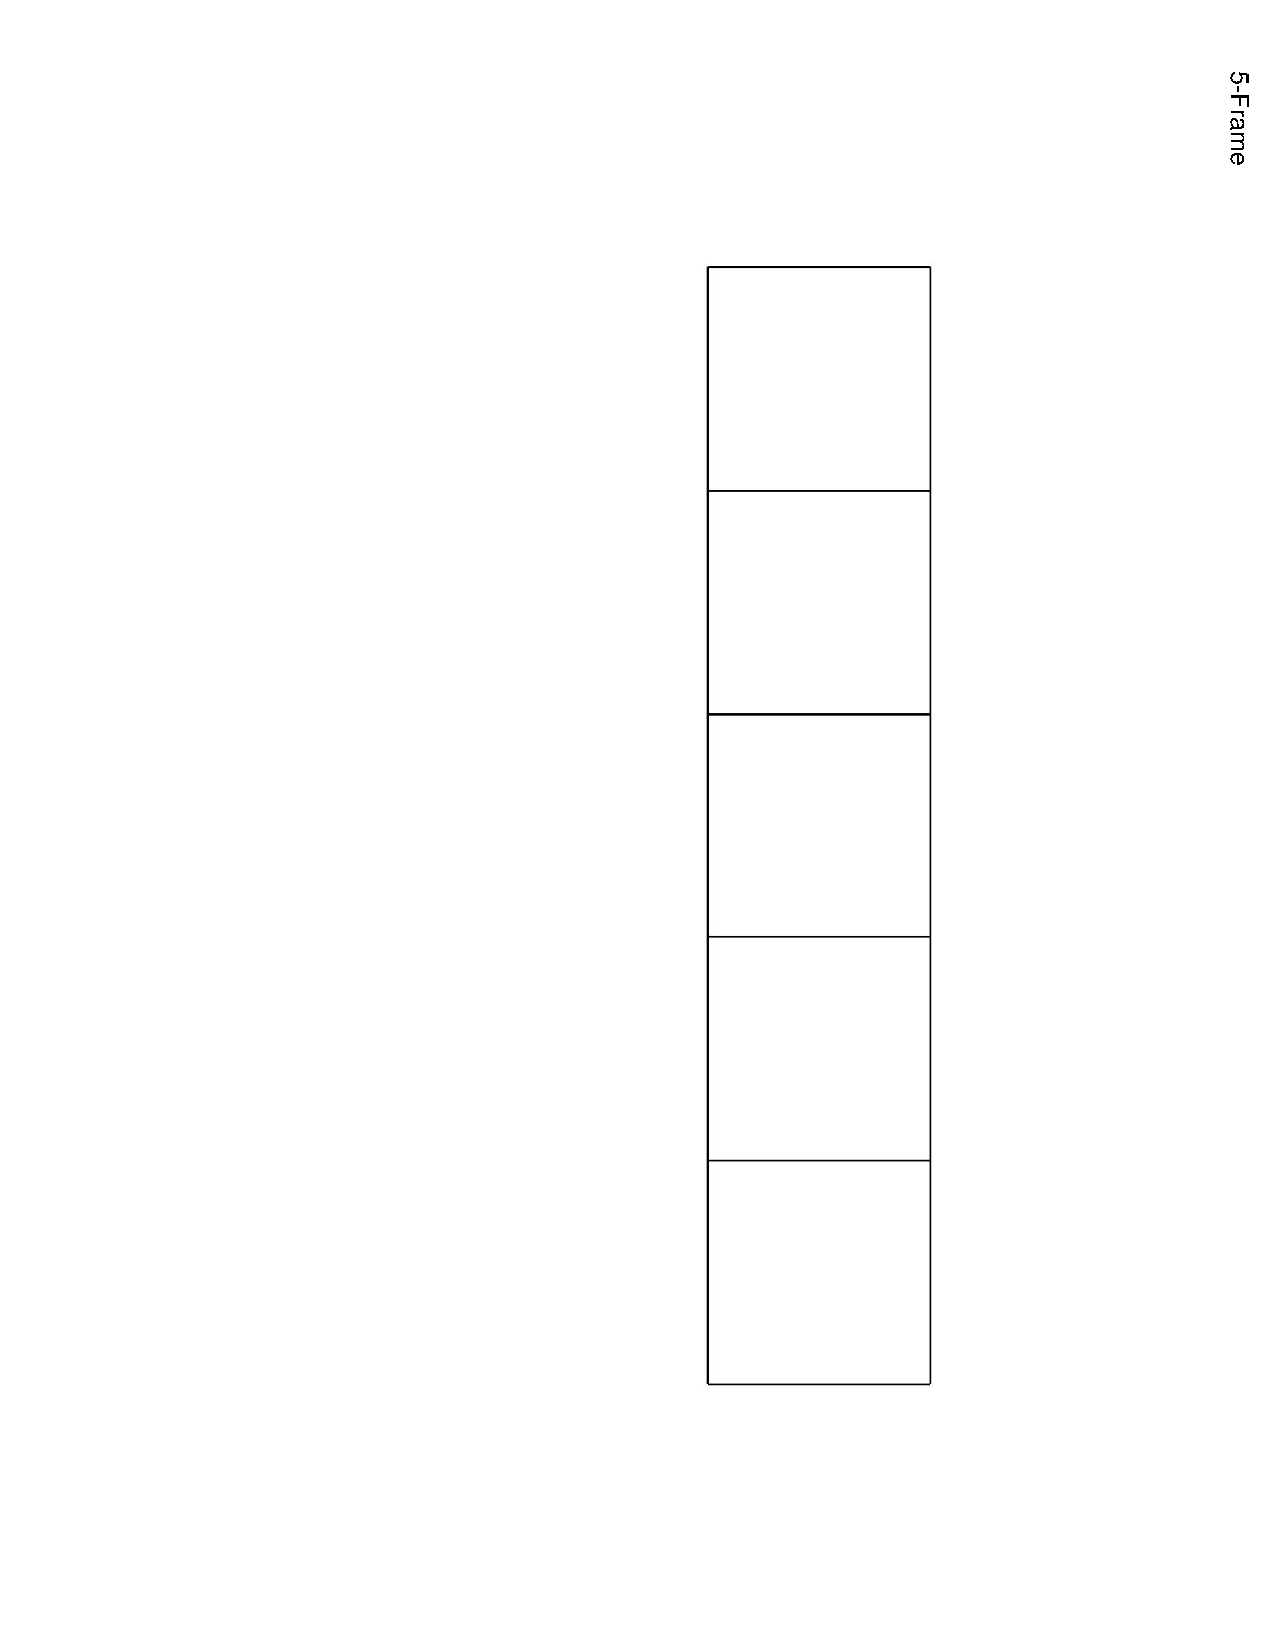
\includegraphics[trim=250 50 100 0, clip, width=0.45\linewidth]{external/blm/pdf-source/tablero-de-5.pdf}
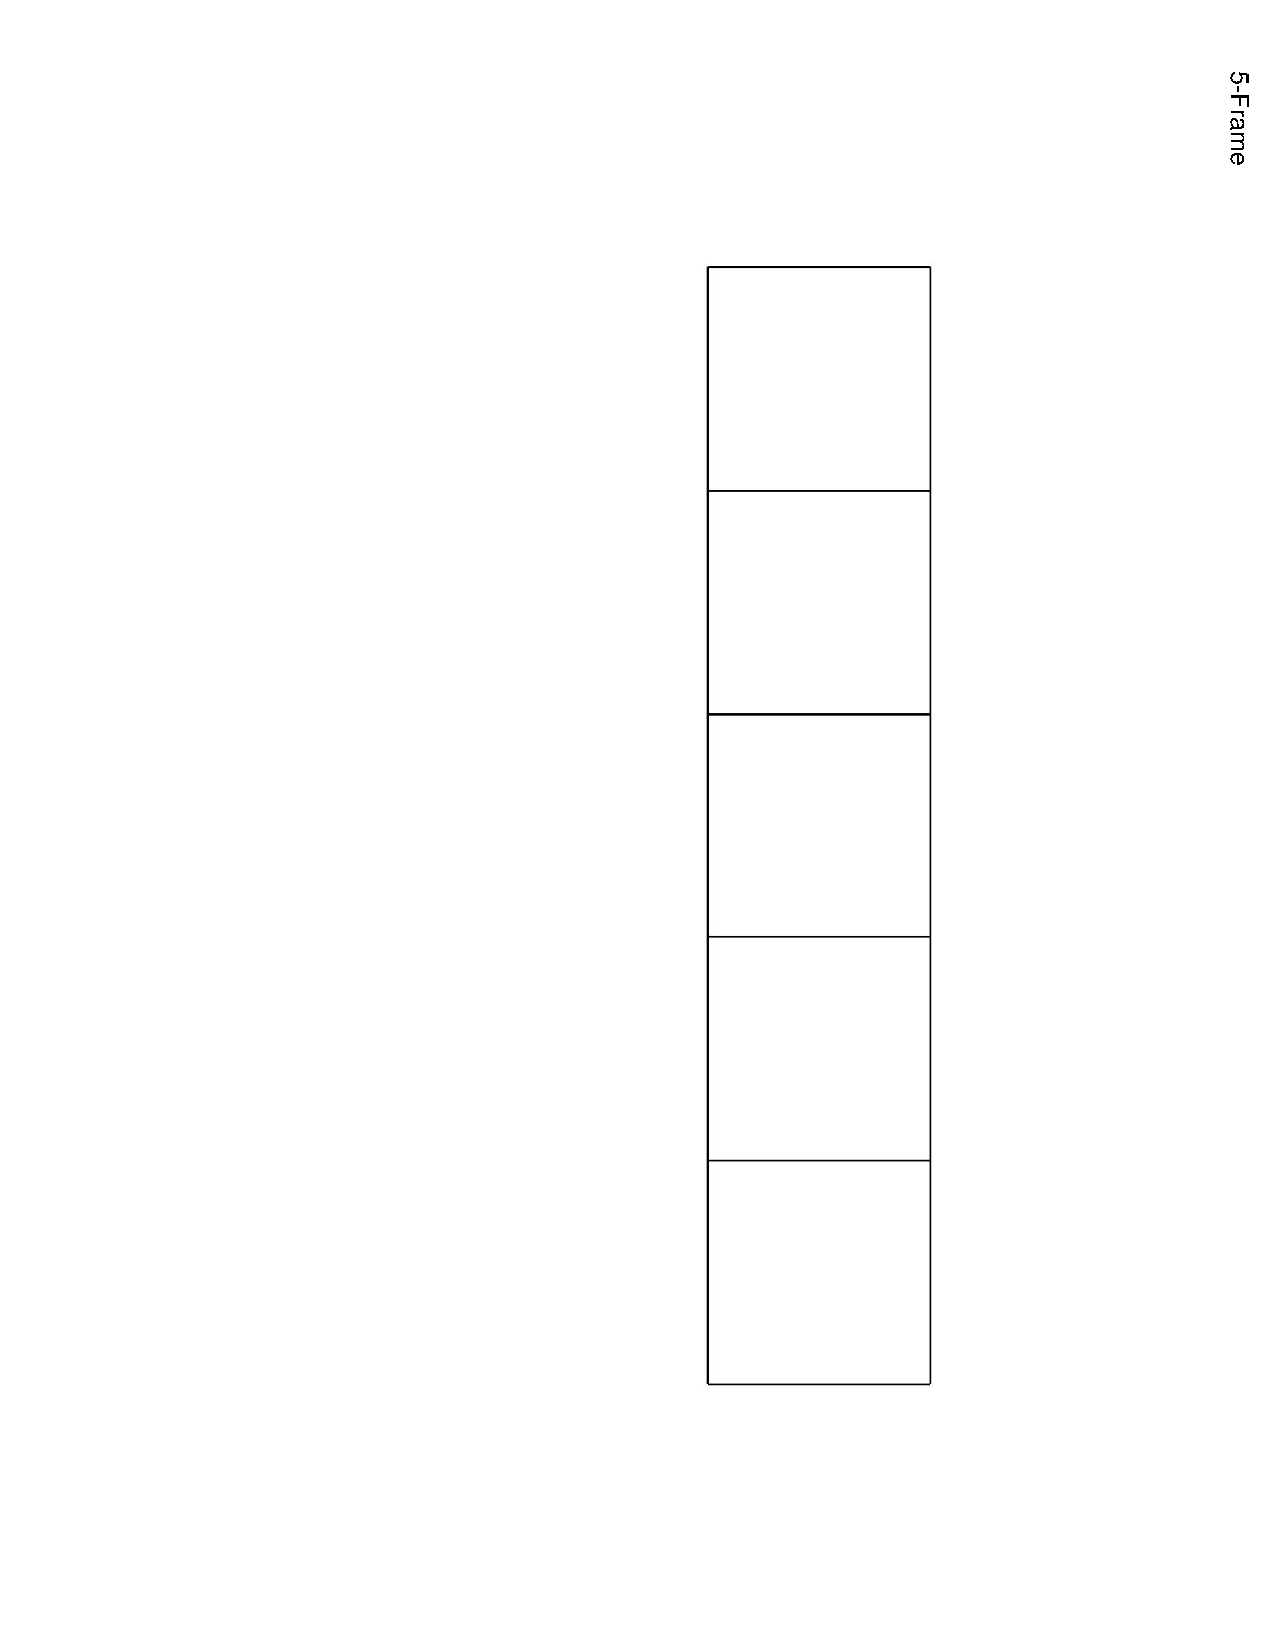
\includegraphics[trim=250 50 100 0, clip, width=0.45\linewidth]{external/blm/pdf-source/tablero-de-5.pdf}
\end{cutoutpage}
\end{activity}%
\end{subsubsectionptx}
\end{subsectionptx}
%
%
\typeout{************************************************}
\typeout{Subsección  Lección 4 -~Exploremos los bloques sólidos geométricos}
\typeout{************************************************}
%
\begin{subsectionptx}{Subsección}{Lección 4 -~Exploremos los bloques sólidos geométricos}{}{Lección 4}{}{}{lec-exploremosBloquesSolidosGeom}
%
%
\typeout{************************************************}
\typeout{Subsubsección  Actividad 2}
\typeout{************************************************}
%
\begin{subsubsectionptx}{Subsubsección}{Actividad 2}{}{Actividad 2}{}{}{lec-exploremosBloquesSolidosGeom-act2}
\begin{activity}{Actividad}{Conozcamos “Bloques sólidos geométricos: Construye lo que ves”.}{act-conozcamos-bloquesSolidosGeom-construyeVes}%
Usa bloques para construir una casa.%
\begin{image}{0}{1}{0}{}%
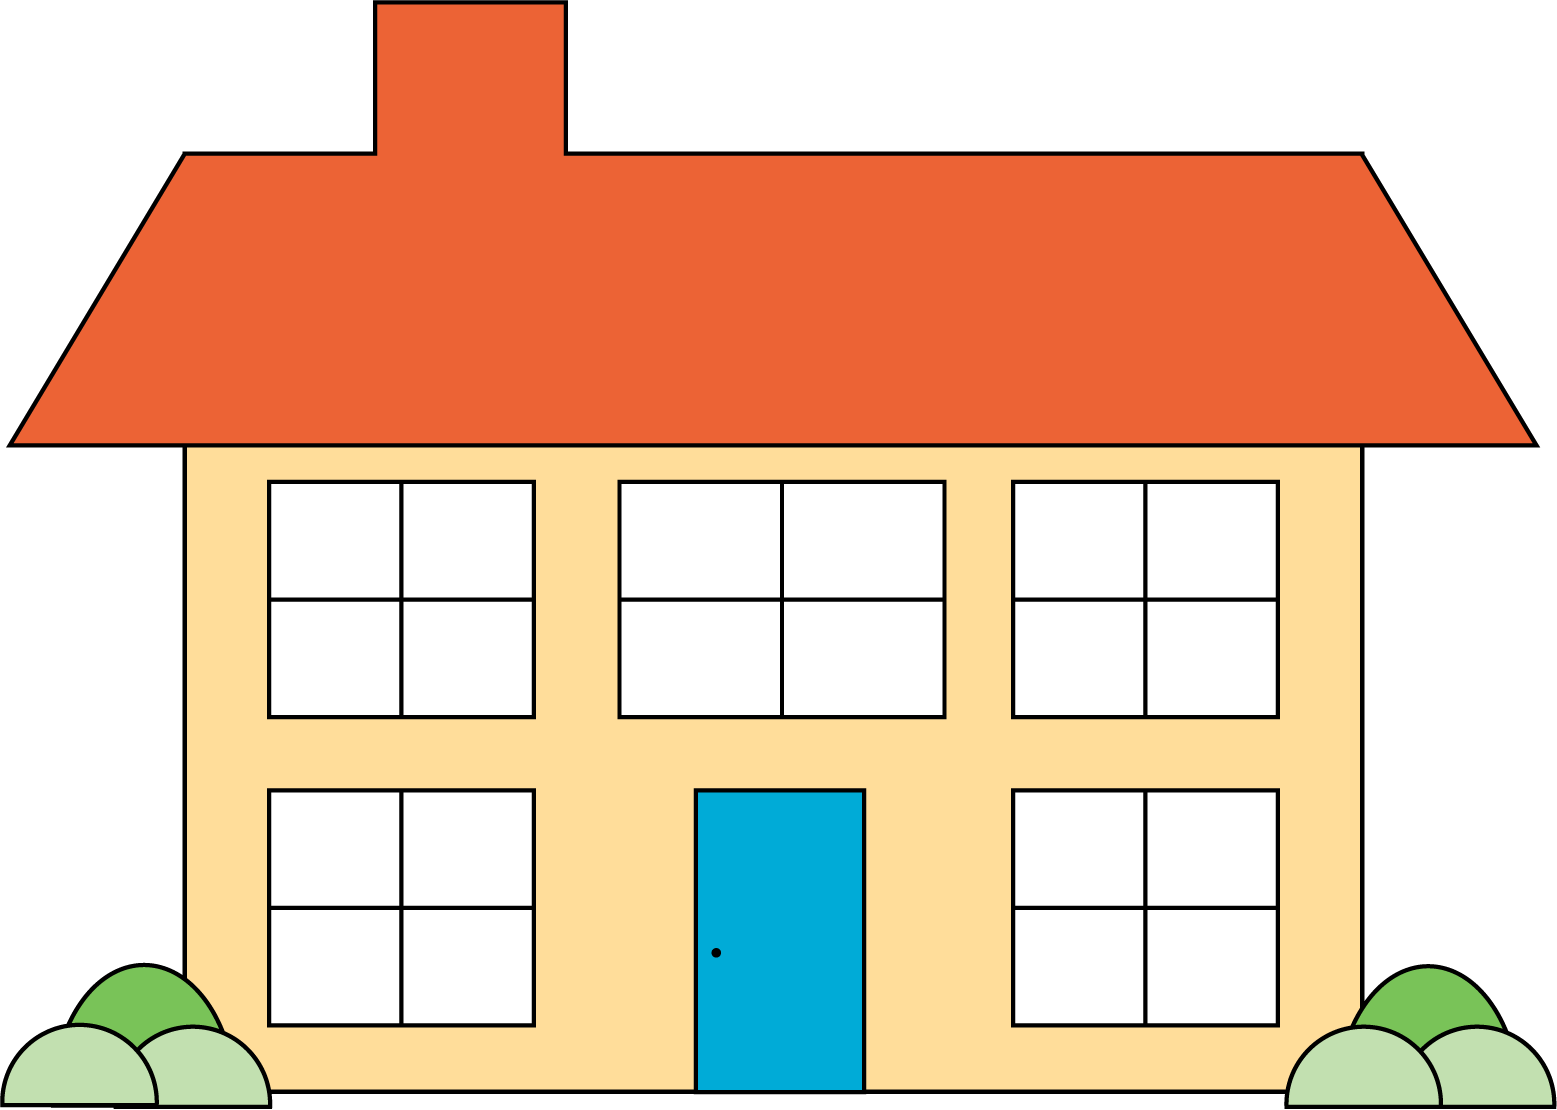
\includegraphics[max width=\linewidth, center]{external/png-source/house.png}
\end{image}%
% Más imágenes al final del libro.%
\begin{cutoutpage}[Tarjetas “Bloques sólidos geométricos: Construye lo que ves”]

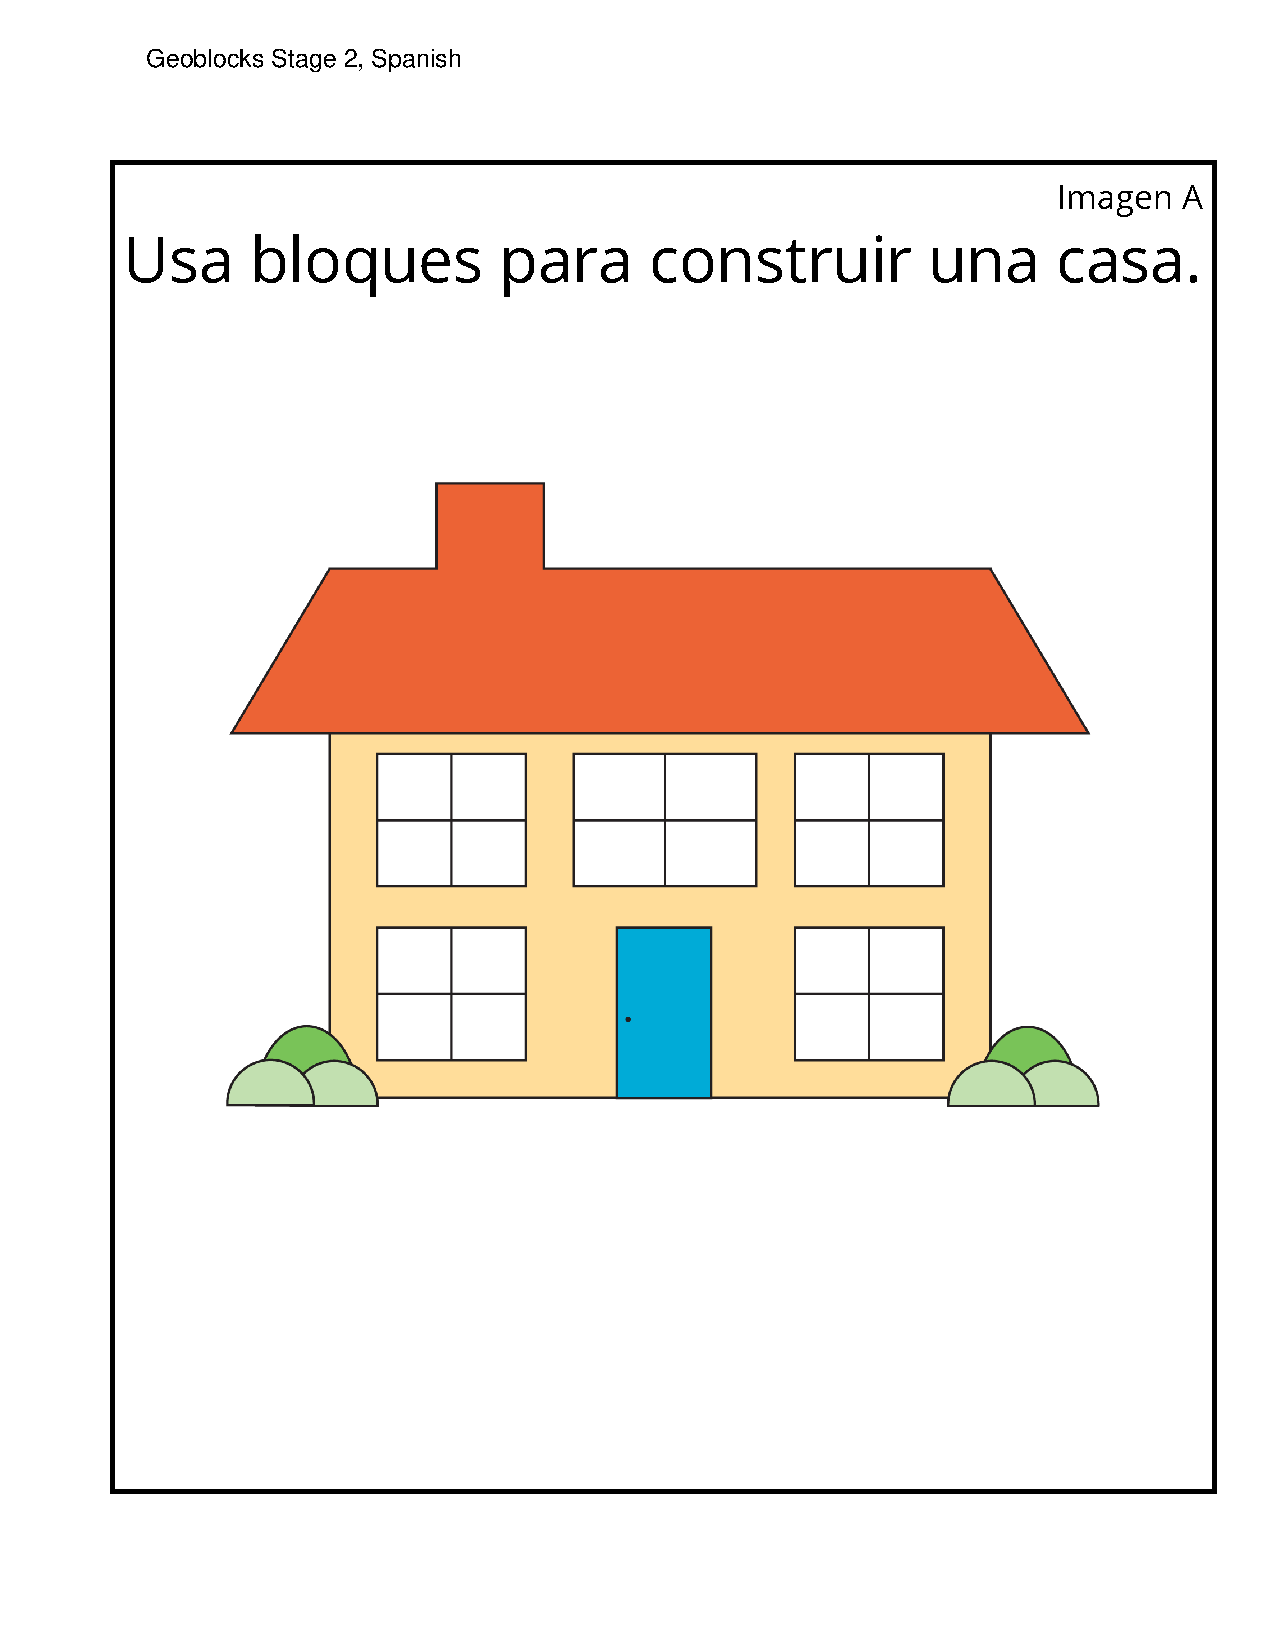
\includegraphics[page=1, trim=60 250 35 80,clip, width=0.7\linewidth, center]{external/blm/pdf-source/bloques-solidos-geometricos-tarjetas.pdf}
\vfill
\noindent\rule{\linewidth}{0.4pt}
\vfill
\includegraphics[page=2, trim=60 250 35 60,clip, width=0.7\linewidth, center]{external/blm/pdf-source/bloques-solidos-geometricos-tarjetas.pdf}
\noindent\rule{\linewidth}{0.4pt}
\cleardoublepage

\includegraphics[page=3, trim=60 250 35 80,clip, width=0.7\linewidth, center]{external/blm/pdf-source/bloques-solidos-geometricos-tarjetas.pdf}
\vfill
\noindent\rule{\linewidth}{0.4pt}
\vfill
\includegraphics[page=4, trim=60 250 35 60,clip, width=0.7\linewidth, center]{external/blm/pdf-source/bloques-solidos-geometricos-tarjetas.pdf}
\noindent\rule{\linewidth}{0.4pt}
\cleardoublepage

\includegraphics[page=5, trim=60 250 35 80,clip, width=0.7\linewidth, center]{external/blm/pdf-source/bloques-solidos-geometricos-tarjetas.pdf}
\vfill
\noindent\rule{\linewidth}{0.4pt}
\vfill
\includegraphics[page=6, trim=60 250 35 60,clip, width=0.7\linewidth, center]{external/blm/pdf-source/bloques-solidos-geometricos-tarjetas.pdf}
\noindent\rule{\linewidth}{0.4pt}
\cleardoublepage

\includegraphics[page=7, trim=60 250 35 80,clip, width=0.7\linewidth, center]{external/blm/pdf-source/bloques-solidos-geometricos-tarjetas.pdf}
\vfill
\noindent\rule{\linewidth}{0.4pt}
\vfill
\includegraphics[page=8, trim=60 250 35 60,clip, width=0.7\linewidth, center]{external/blm/pdf-source/bloques-solidos-geometricos-tarjetas.pdf}
\noindent\rule{\linewidth}{0.4pt}
\cleardoublepage

\includegraphics[page=9, trim=60 250 35 90,clip, width=0.7\linewidth, center]{external/blm/pdf-source/bloques-solidos-geometricos-tarjetas.pdf}
\vfill
\noindent\rule{\linewidth}{0.4pt}
\vfill
\includegraphics[page=10, trim=60 250 35 60,clip, width=0.7\linewidth, center]{external/blm/pdf-source/bloques-solidos-geometricos-tarjetas.pdf}
\noindent\rule{\linewidth}{0.4pt}
\end{cutoutpage}
\end{activity}%
\end{subsubsectionptx}
\end{subsectionptx}
%
%
\typeout{************************************************}
\typeout{Subsección  Lección 5 -~Exploremos nuestras herramientas matemáticas}
\typeout{************************************************}
%
\begin{subsectionptx}{Subsección}{Lección 5 -~Exploremos nuestras herramientas matemáticas}{}{Lección 5}{}{}{lec-exploremosHerramientasMate}
%
%
\typeout{************************************************}
\typeout{Subsubsección  Actividad 1}
\typeout{************************************************}
%
\begin{subsubsectionptx}{Subsubsección}{Actividad 1}{}{Actividad 1}{}{}{lec-exploremosHerramientasMate-act1}
\begin{activity}{Actividad}{Conozcamos “Cubos encajables: Construye lo que ves”.}{act-conozcamos-construyeLoQueVes}%
\begin{image}{0}{1}{0}{-1\baselineskip}%
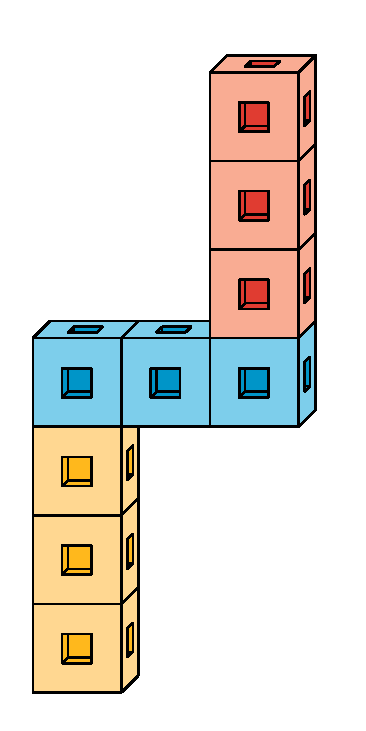
\includegraphics[max width=0.2\linewidth, center]{external/svg-source/tikz-file-148146.pdf}
\end{image}%
\begin{cutoutpage}[tarjetas para “Cubos encajables: Construye lo que ves”]
% 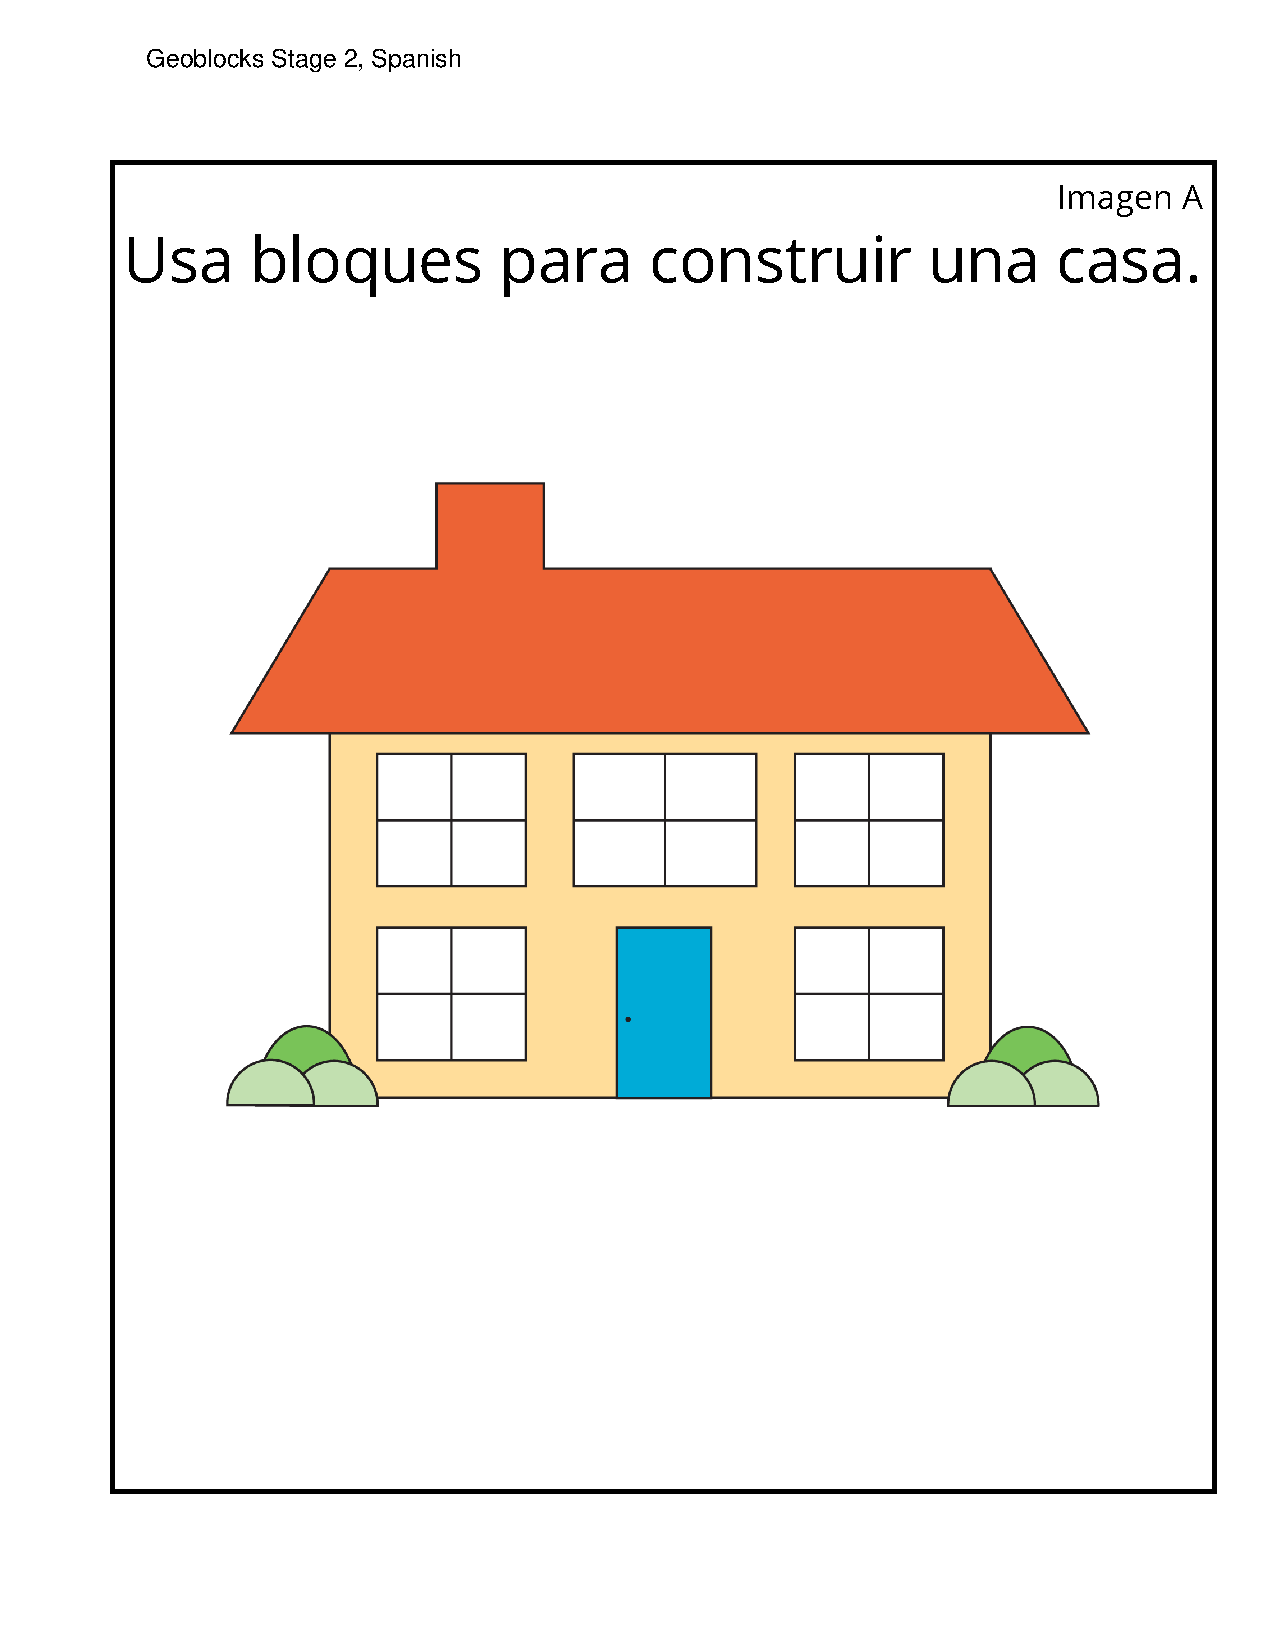
\includegraphics[page=1, trim=60 250 35 80,clip, width=0.7\linewidth, center]{external/blm/pdf-source/bloques-solidos-geometricos-tarjetas.pdf}
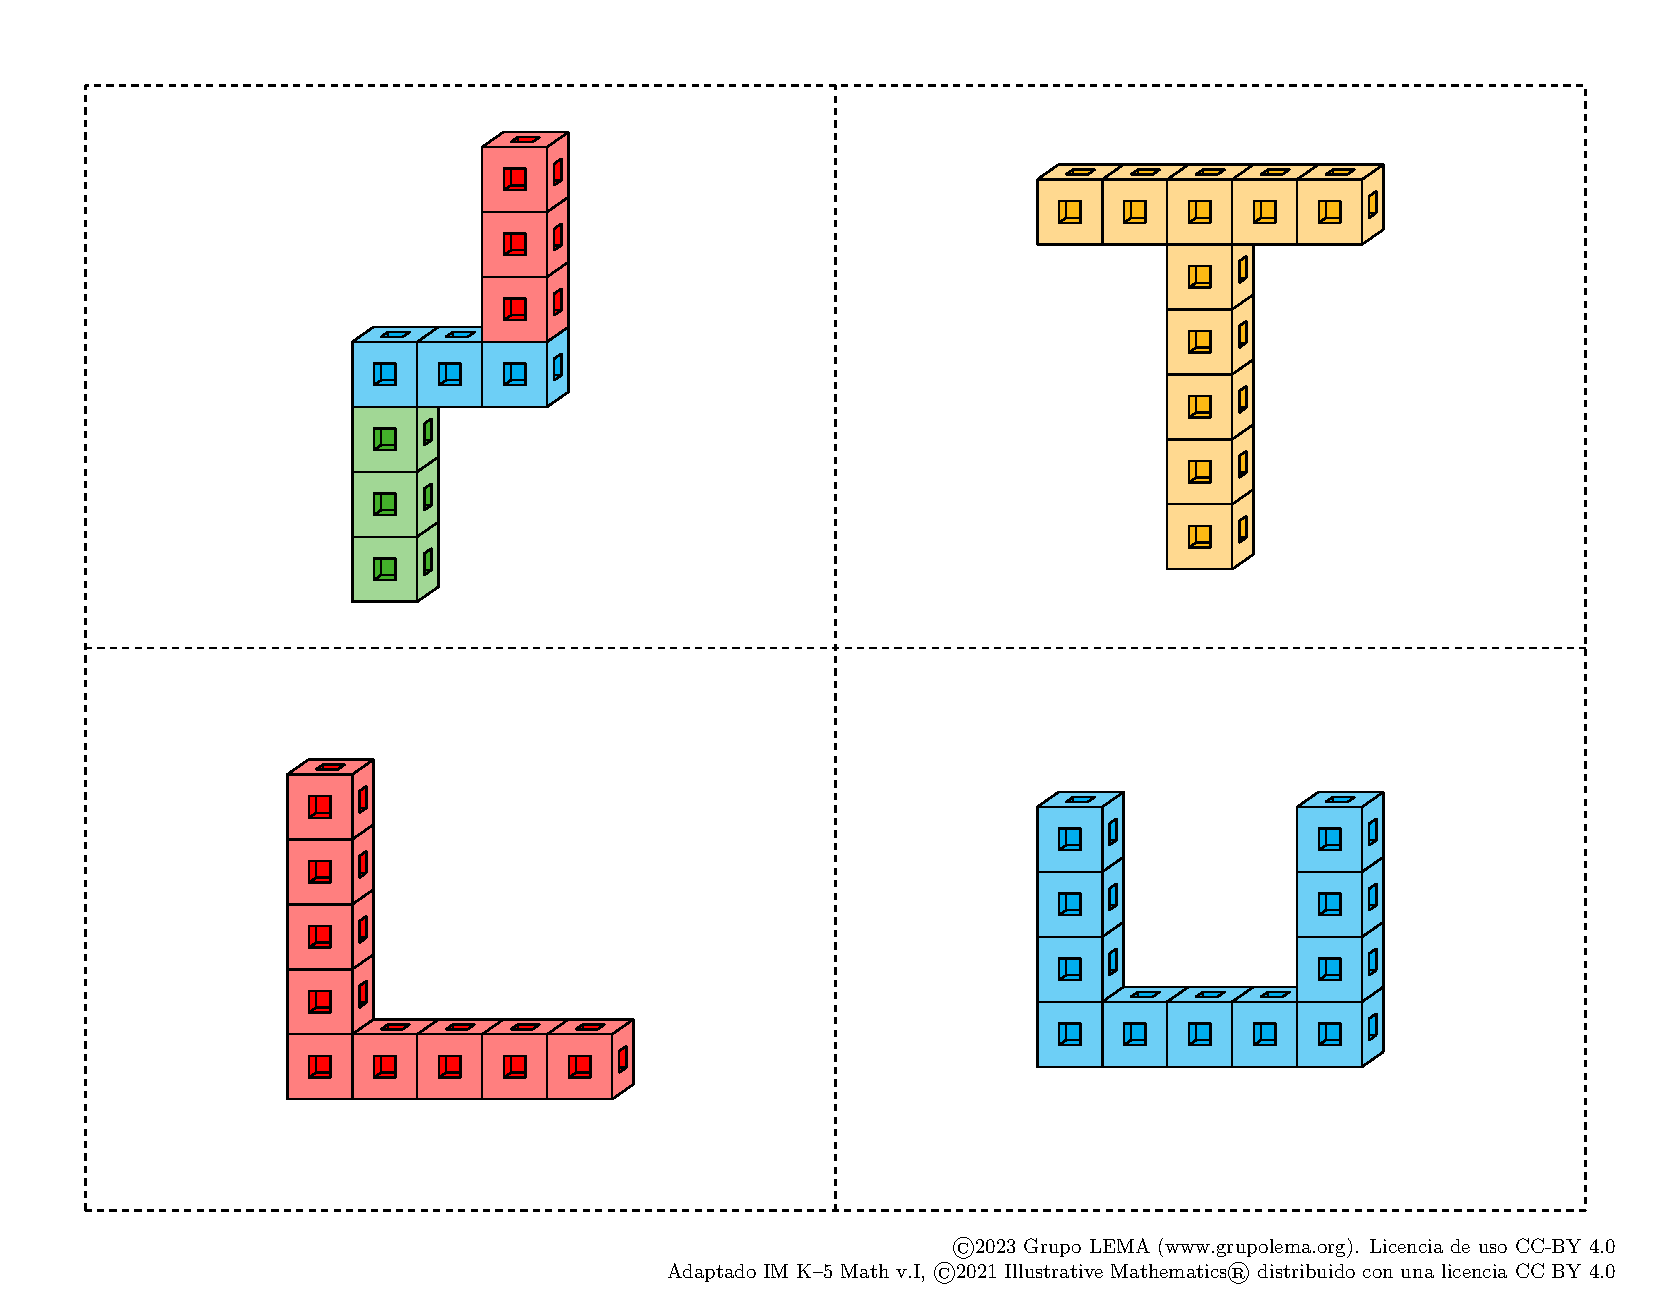
\includegraphics[page=1, rotate=90, width=1.1\linewidth, center]{external/blm/tikz-source/cubos-encajables-tarjetas.pdf}
\cleardoublepage
\includegraphics[page=2, rotate=90, width=1.1\linewidth, center]{external/blm/tikz-source/cubos-encajables-tarjetas.pdf}
\cleardoublepage
\includegraphics[page=3, rotate=90, width=1.1\linewidth, center]{external/blm/tikz-source/cubos-encajables-tarjetas.pdf}
\end{cutoutpage}
\end{activity}%
\end{subsubsectionptx}
%
%
\typeout{************************************************}
\typeout{Subsubsección  Actividad 2}
\typeout{************************************************}
%
\begin{subsubsectionptx}{Subsubsección}{Actividad 2}{}{Actividad 2}{}{}{lec-exploremosHerramientasMate-act2}
\begin{activity}{Actividad}{Conozcamos “Fichas geométricas: Rompecabezas”.}{act-conozcamos-fichasGeometricas-rompecabezas}%
\begin{image}{0}{1}{0}{-1\baselineskip}%

\includegraphics[max width=0.3\linewidth, center]{external/svg-source/tikz-file-148147.pdf}
\end{image}%
\end{activity}%
\begin{cutoutpage}[Tarjetas para “Fichas geométricas: Rompecabezas” (laminar por ambos lados)]
% 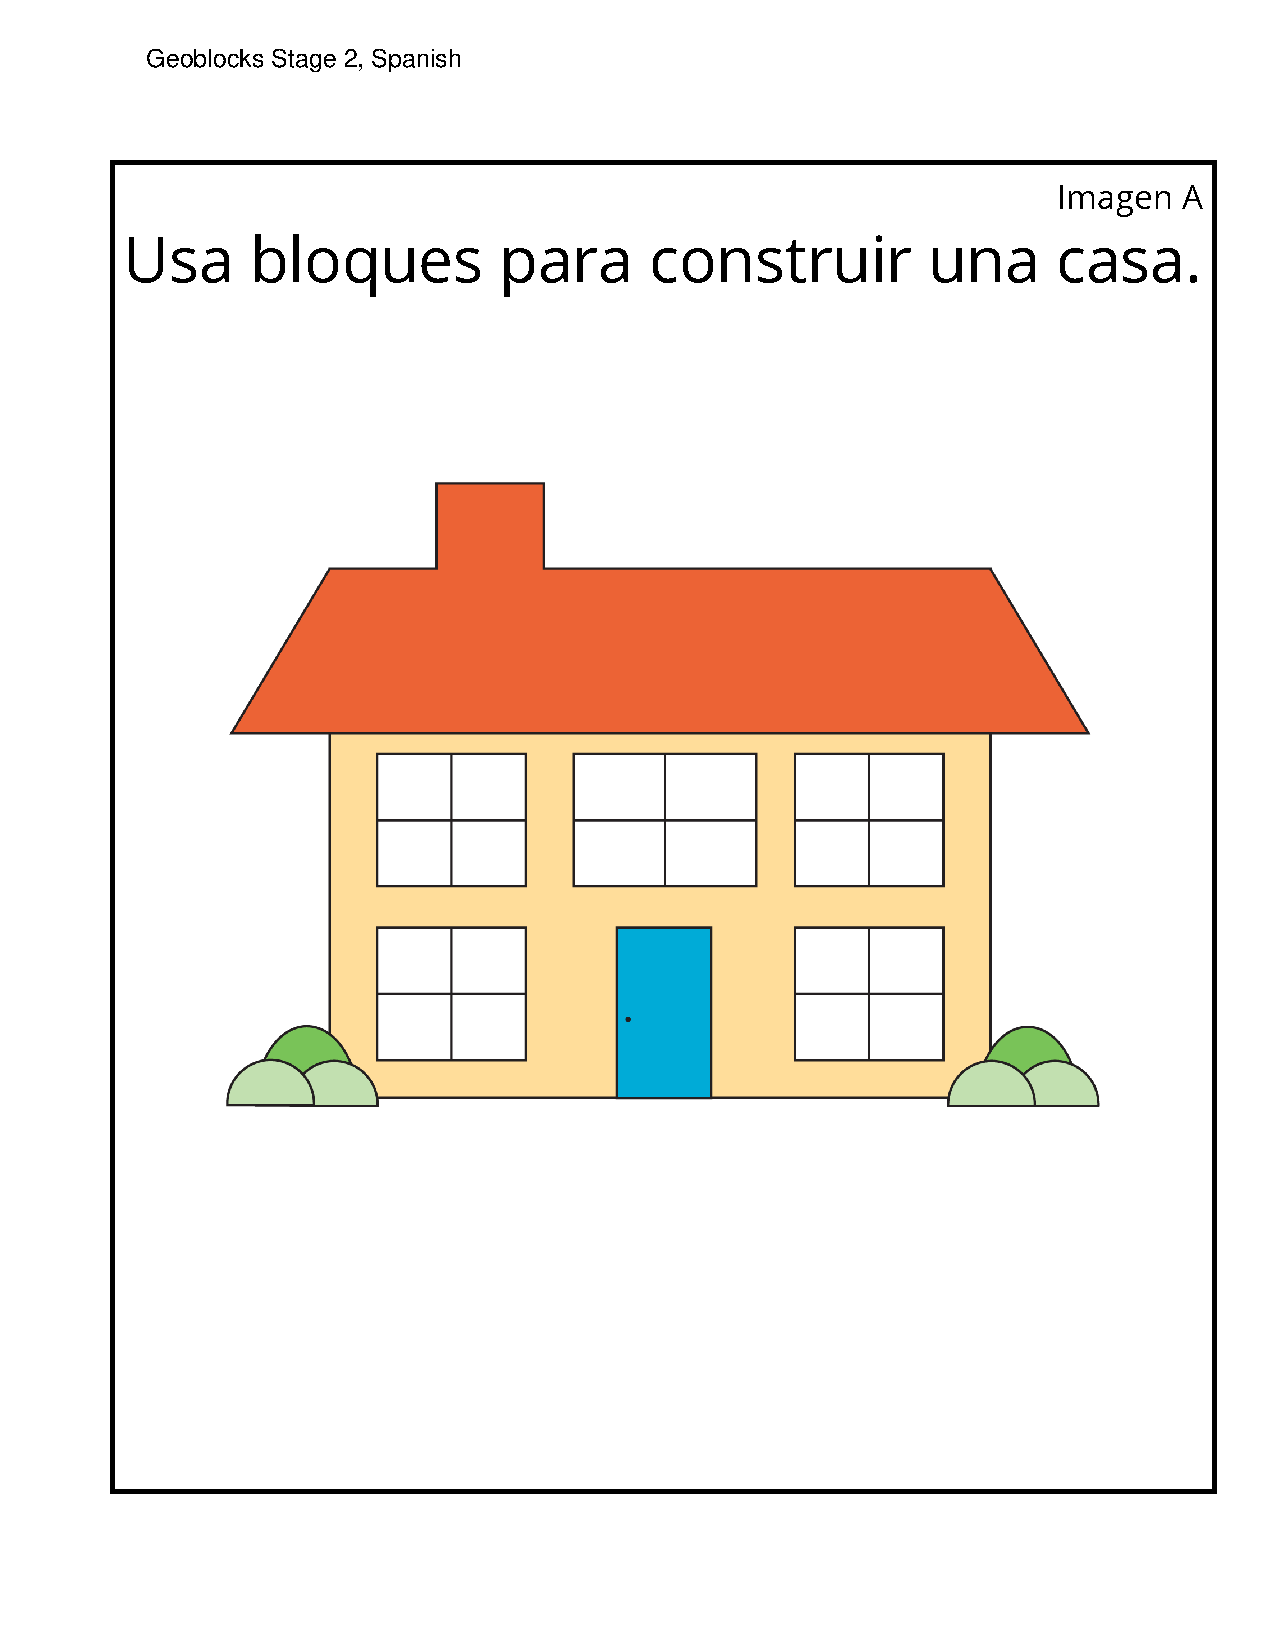
\includegraphics[page=1, trim=60 250 35 80,clip, width=0.7\linewidth, center]{external/blm/pdf-source/bloques-solidos-geometricos-tarjetas.pdf}
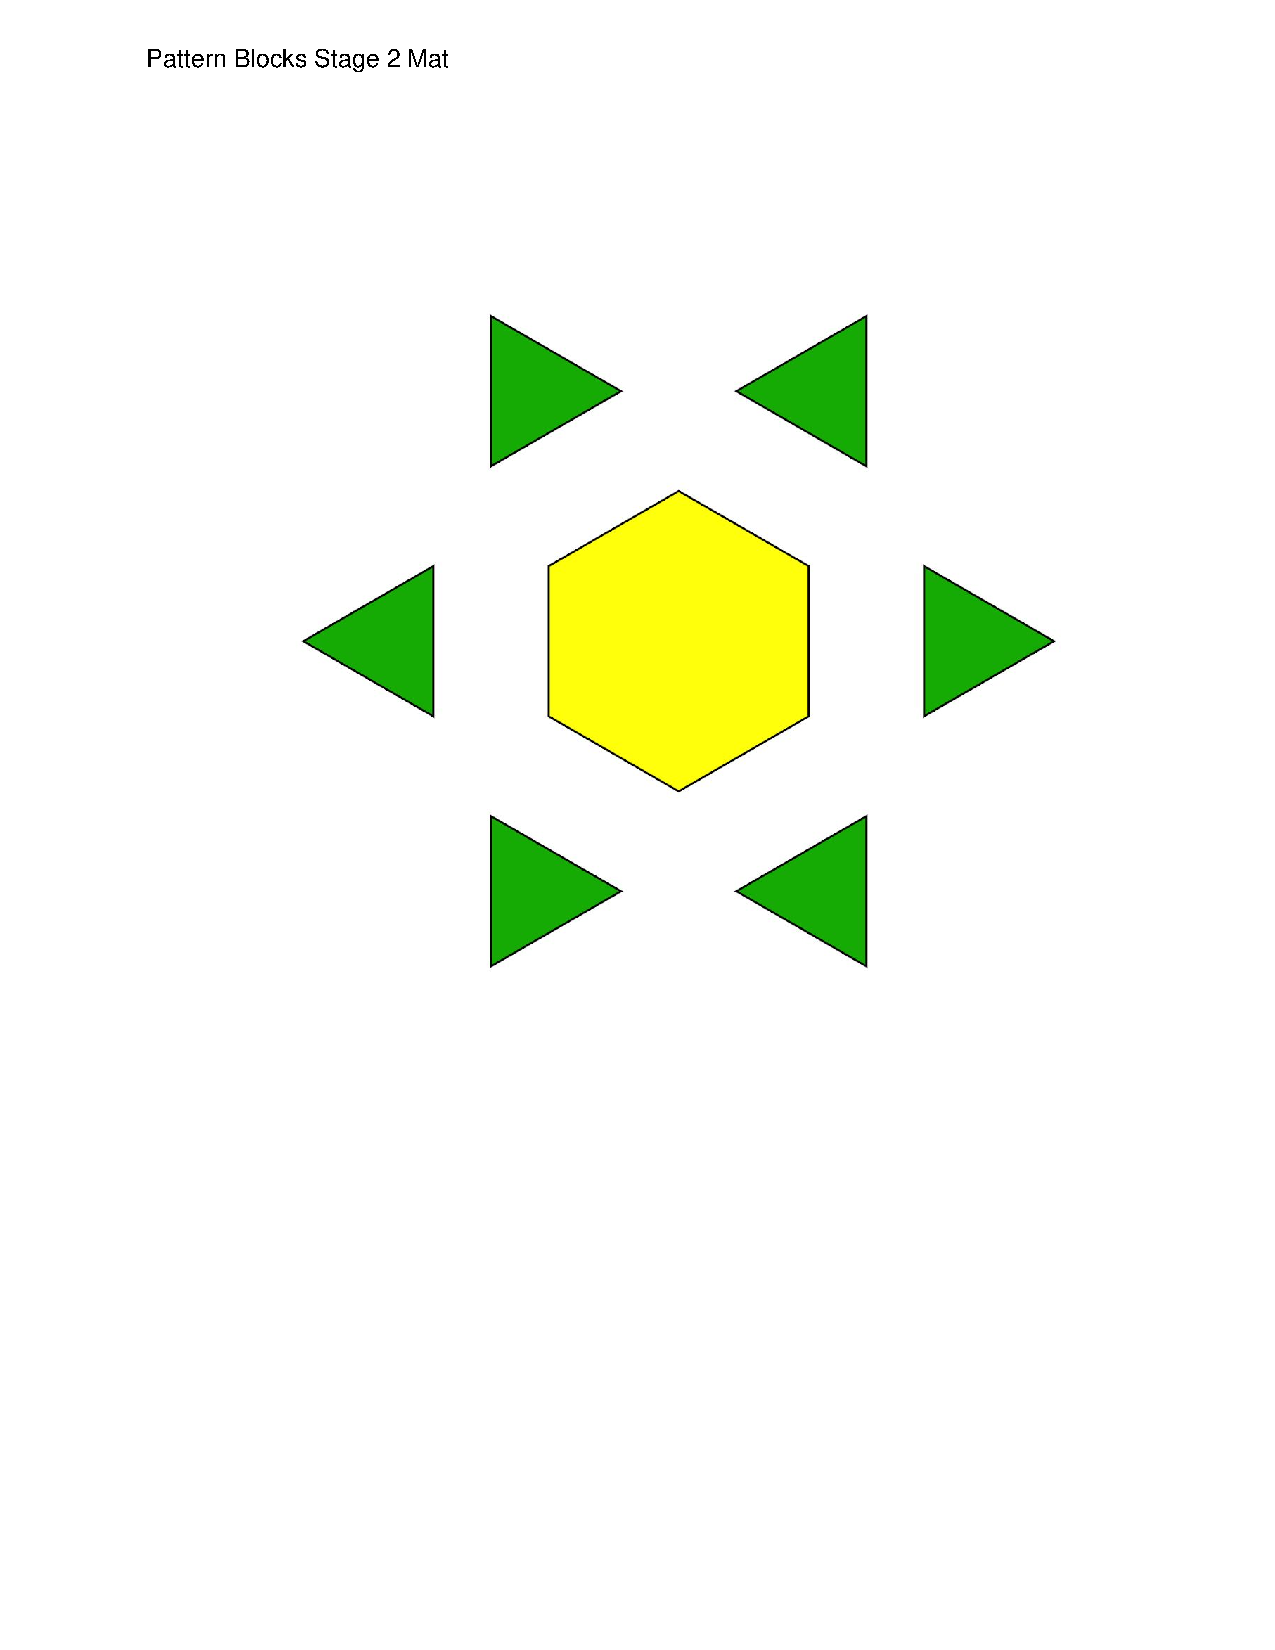
\includegraphics[page=1, trim=0 0 0 40, clip, width=\linewidth, center]{external/blm/pdf-source/fichasGeometricas-rompecabezas.pdf}
\clearpage
\includegraphics[page=2, trim=0 0 0 40, clip, width=\linewidth, center]{external/blm/pdf-source/fichasGeometricas-rompecabezas.pdf}
\clearpage
\includegraphics[page=3, trim=0 0 0 40, clip, width=\linewidth, center]{external/blm/pdf-source/fichasGeometricas-rompecabezas.pdf}
\clearpage
\includegraphics[page=4, trim=0 0 0 40, clip, width=\linewidth, center]{external/blm/pdf-source/fichasGeometricas-rompecabezas.pdf}
\clearpage
\includegraphics[page=5, trim=0 0 0 40, clip, width=\linewidth, center]{external/blm/pdf-source/fichasGeometricas-rompecabezas.pdf}
\clearpage
\includegraphics[page=6, trim=0 0 0 40, clip, width=\linewidth, center]{external/blm/pdf-source/fichasGeometricas-rompecabezas.pdf}
\clearpage
\includegraphics[page=7, trim=0 0 0 40, clip, width=\linewidth, center]{external/blm/pdf-source/fichasGeometricas-rompecabezas.pdf}
\clearpage
\includegraphics[page=8, trim=0 0 0 40, clip, width=\linewidth, center]{external/blm/pdf-source/fichasGeometricas-rompecabezas.pdf}
\clearpage
\includegraphics[page=9, trim=0 0 0 40, clip, width=\linewidth, center]{external/blm/pdf-source/fichasGeometricas-rompecabezas.pdf}
\clearpage
\includegraphics[page=10, trim=0 0 0 40, clip, width=\linewidth, center]{external/blm/pdf-source/fichasGeometricas-rompecabezas.pdf}
\end{cutoutpage}
\end{subsubsectionptx}
\end{subsectionptx}
\end{sectionptx}
%
%
\typeout{************************************************}
\typeout{Sección  Sección B -~Reconozcamos cantidades}
\typeout{************************************************}
%
\begin{sectionptx}{Sección}{Sección B -~Reconozcamos cantidades}{}{Sección B -~Reconozcamos cantidades}{}{}{gra0-uni1-secB}
%
%
\typeout{************************************************}
\typeout{Subsección  Lección 6 -~Busquemos grupos pequeños}
\typeout{************************************************}
%
\begin{subsectionptx}{Subsección}{Lección 6 -~Busquemos grupos pequeños}{}{Lección 6}{}{}{lec-busquemosGruposMasPequenos}
\end{subsectionptx}
%
%
\typeout{************************************************}
\typeout{Subsección  Lección 7 -~Juego de búsqueda en el salón de clase}
\typeout{************************************************}
%
\begin{subsectionptx}{Subsección}{Lección 7 -~Juego de búsqueda en el salón de clase}{}{Lección 7}{}{}{lec-juegoBusqueda}
\end{subsectionptx}
%
%
\typeout{************************************************}
\typeout{Subsección  Lección 8 -~Grupos diferentes, misma cantidad}
\typeout{************************************************}
%
\begin{subsectionptx}{Subsección}{Lección 8 -~Grupos diferentes, misma cantidad}{}{Lección 8}{}{}{lec-gruposDiferentesMismaCantidad}
%
%
\typeout{************************************************}
\typeout{Subsubsección  Actividad 2}
\typeout{************************************************}
%
\begin{subsubsectionptx}{Subsubsección}{Actividad 2}{}{Actividad 2}{}{}{lec-gruposDiferentesMismaCantidad-act2}
\begin{activity}{Actividad}{Grupos diferentes, misma cantidad.}{act-gruposDiferentesMismaCantidad}%
\begin{image}{0}{1}{0}{}%
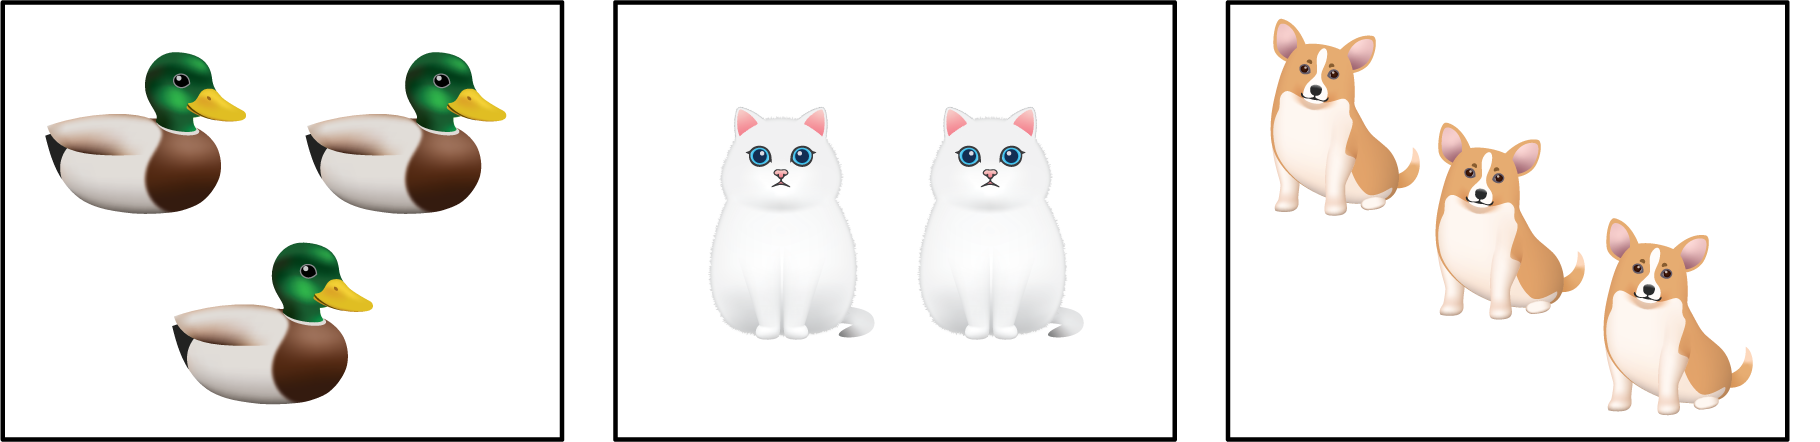
\includegraphics[max width=\linewidth, center]{external/png-source/K.1.C Beta Student Workbook.AnimalGroups.png}
\end{image}%
\begin{cutoutpage}[Tarjetas para "Grupos diferentes, misma cantidad" (recortar)]
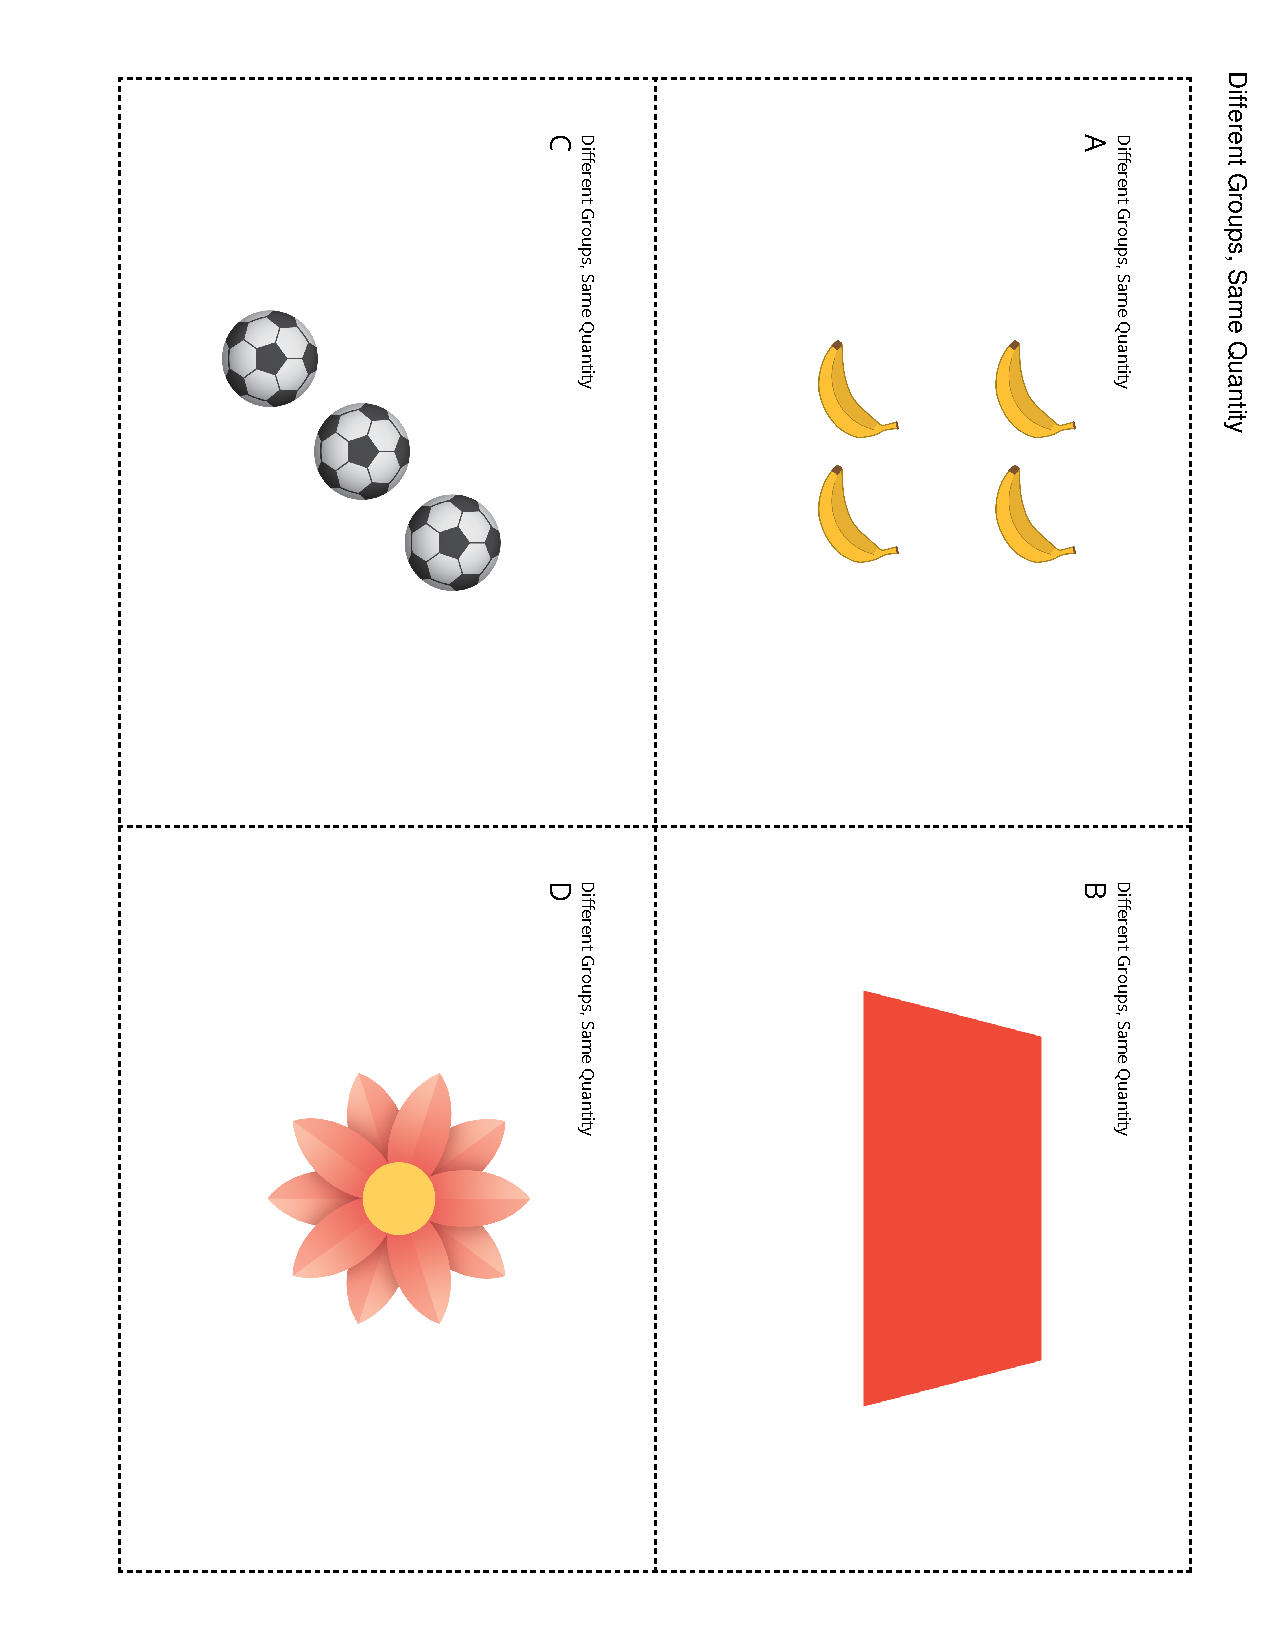
\includegraphics[page=1, trim=55 35 35 0, clip, width=\linewidth, center]{external/blm/pdf-source/gruposDiferentesMismaCantidad.pdf}
\cleardoublepage
\includegraphics[page=2, trim=55 35 35 0, clip, width=\linewidth, center]{external/blm/pdf-source/gruposDiferentesMismaCantidad.pdf}
\cleardoublepage
\end{cutoutpage}
\end{activity}%
\end{subsubsectionptx}
\end{subsectionptx}
%
%
\typeout{************************************************}
\typeout{Subsección  Lección 9 -~Hagamos libros de imágenes}
\typeout{************************************************}
%
\begin{subsectionptx}{Subsección}{Lección 9 -~Hagamos libros de imágenes}{}{Lección 9}{}{}{lec-hagamosDeLibrosImagenes}
%
%
\typeout{************************************************}
\typeout{Subsubsección  Actividad 2}
\typeout{************************************************}
%
\begin{subsubsectionptx}{Subsubsección}{Actividad 2}{}{Actividad 2}{}{}{lec-hagamosDeLibrosImagenes-act2}
\begin{activity}{Actividad}{Conozcamos “Libros de imágenes: Crea”.}{act-conozcamos-librosDeImagenes-crea}%
Hojas del libro para crear en las páginas que siguen.
\end{activity}%
\clearpage

\includegraphics[page=2, rotate=90, trim=90 35 35 35, clip, width=\linewidth, center]{external/blm/pdf-source/center-picture-books-k-5-stage-2-create-picture-books-stage-2-recording-sheet.pdf}
\hrule

\includegraphics[page=1, rotate=90, trim=90 35 35 35, clip, width=\linewidth, center]{external/blm/pdf-source/center-picture-books-k-5-stage-2-create-picture-books-stage-2-recording-sheet.pdf}
\clearpage

\includegraphics[page=4, rotate=90, trim=90 35 35 35, clip, width=\linewidth, center]{external/blm/pdf-source/center-picture-books-k-5-stage-2-create-picture-books-stage-2-recording-sheet.pdf}
\hrule

\includegraphics[page=3, rotate=90, trim=90 35 35 35, clip, width=\linewidth, center]{external/blm/pdf-source/center-picture-books-k-5-stage-2-create-picture-books-stage-2-recording-sheet.pdf}
\end{subsubsectionptx}
\end{subsectionptx}
\end{sectionptx}
%
%
\typeout{************************************************}
\typeout{Sección  Sección C -~¿Hay suficientes?}
\typeout{************************************************}
%
\begin{sectionptx}{Sección}{Sección C -~¿Hay suficientes?}{}{Sección C -~¿Hay suficientes?}{}{}{gra0-uni1-secC}
%
%
\typeout{************************************************}
\typeout{Subsección  Lección 10 -~Cuántos ves: Construyamos sobre lo aprendido}
\typeout{************************************************}
%
\begin{subsectionptx}{Subsección}{Lección 10 -~Cuántos ves: Construyamos sobre lo aprendido}{}{Lección 10}{}{}{lec-cuantosVesConstruyamosSobreLoAprendido}
\end{subsectionptx}
%
%
\typeout{************************************************}
\typeout{Subsección  Lección 11 -~Consigamos suficientes}
\typeout{************************************************}
%
\begin{subsectionptx}{Subsección}{Lección 11 -~Consigamos suficientes}{}{Lección 11}{}{}{lec-consigamosSuficientes}
\end{subsectionptx}
\end{sectionptx}
%
%
\typeout{************************************************}
\typeout{Sección  Sección D -~Contemos colecciones}
\typeout{************************************************}
%
\begin{sectionptx}{Sección}{Sección D -~Contemos colecciones}{}{Sección D -~Contemos colecciones}{}{}{gra0-uni1-secD}
%
%
\typeout{************************************************}
\typeout{Subsección  Lección 12 -~¿Cuántos hay? (Parte 1)}
\typeout{************************************************}
%
\begin{subsectionptx}{Subsección}{Lección 12 -~¿Cuántos hay? (Parte 1)}{}{Lección 12}{}{}{lec-cuantosHayParte1}
%
%
\typeout{************************************************}
\typeout{Subsubsección  Actividad 1}
\typeout{************************************************}
%
\begin{subsubsectionptx}{Subsubsección}{Actividad 1}{}{Actividad 1}{}{}{lec-cuantosHayParte1-act1}
\begin{activity}{Actividad}{Contemos colecciones.}{act-contemosColecciones}%
¿Cuántos objetos hay en la colección?%
\par
\begin{cutoutpage}[tablero de conteo (laminar)]
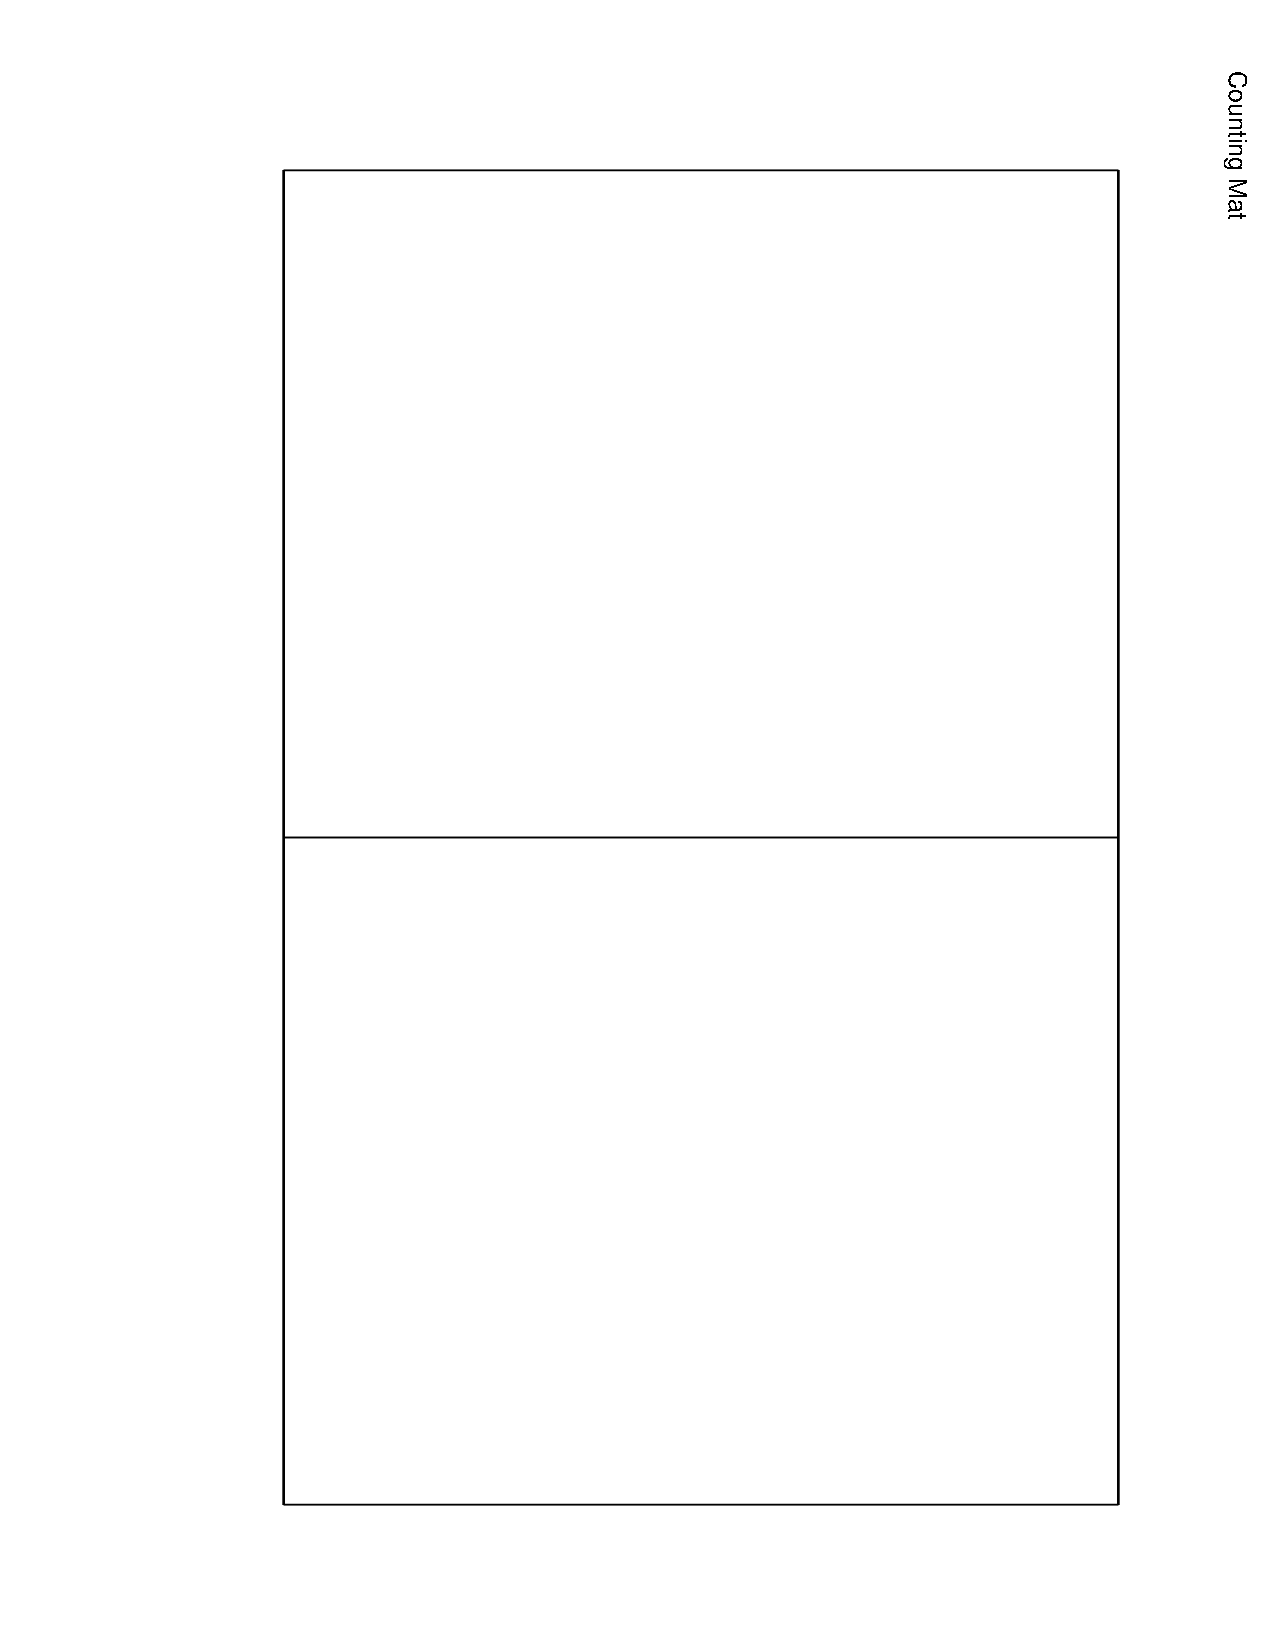
\includegraphics[trim=100 70 50 60, clip, width=\linewidth, center]{external/blm/pdf-source/contemosColecciones-tableroDeConteo-countingMat.pdf}

\end{cutoutpage}
\end{activity}%
\end{subsubsectionptx}
%
%
% \typeout{************************************************}
% \typeout{Subsubsección  Actividad 2}
% \typeout{************************************************}
% %
% \begin{subsubsectionptx}{Subsubsección}{Actividad 2}{}{Actividad 2}{}{}{lec-cuantosHayParte1-act2}
% \begin{activity}{Actividad}{Contemos hasta 10 [Opcional].}{act-contemosHasta10}%
% Contemos juntos hasta 10%
% \end{activity}%
% \end{subsubsectionptx}
\typeout{************************************************}
\typeout{Subsubsección  Actividad 3}
\typeout{************************************************}
%
\begin{subsubsectionptx}{Subsubsección}{Actividad 3}{}{Actividad 3}{}{}{lec-cuantosHayParte1-act3}
\begin{activity}{Actividad}{Conozcamos “Fichas geométricas: Consigue y construye”.}{act-conozcamos-fichasGeometricas-consigueYConstruye}%
\begin{image}{0}{1}{0}{}%
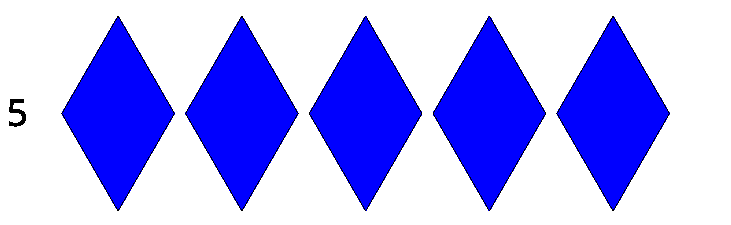
\includegraphics[width=\linewidth]{external/svg-source/tikz-file-148183.pdf}
\end{image}%
\begin{image}{0}{1}{0}{}%
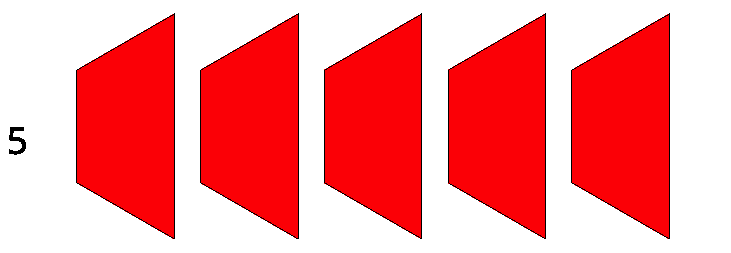
\includegraphics[width=\linewidth]{external/svg-source/tikz-file-148184.pdf}
\end{image}%
\begin{cutoutpage}[Tarjetas para Fichas geométricas: “Fichas geométricas: Consigue y construye” (laminar)]
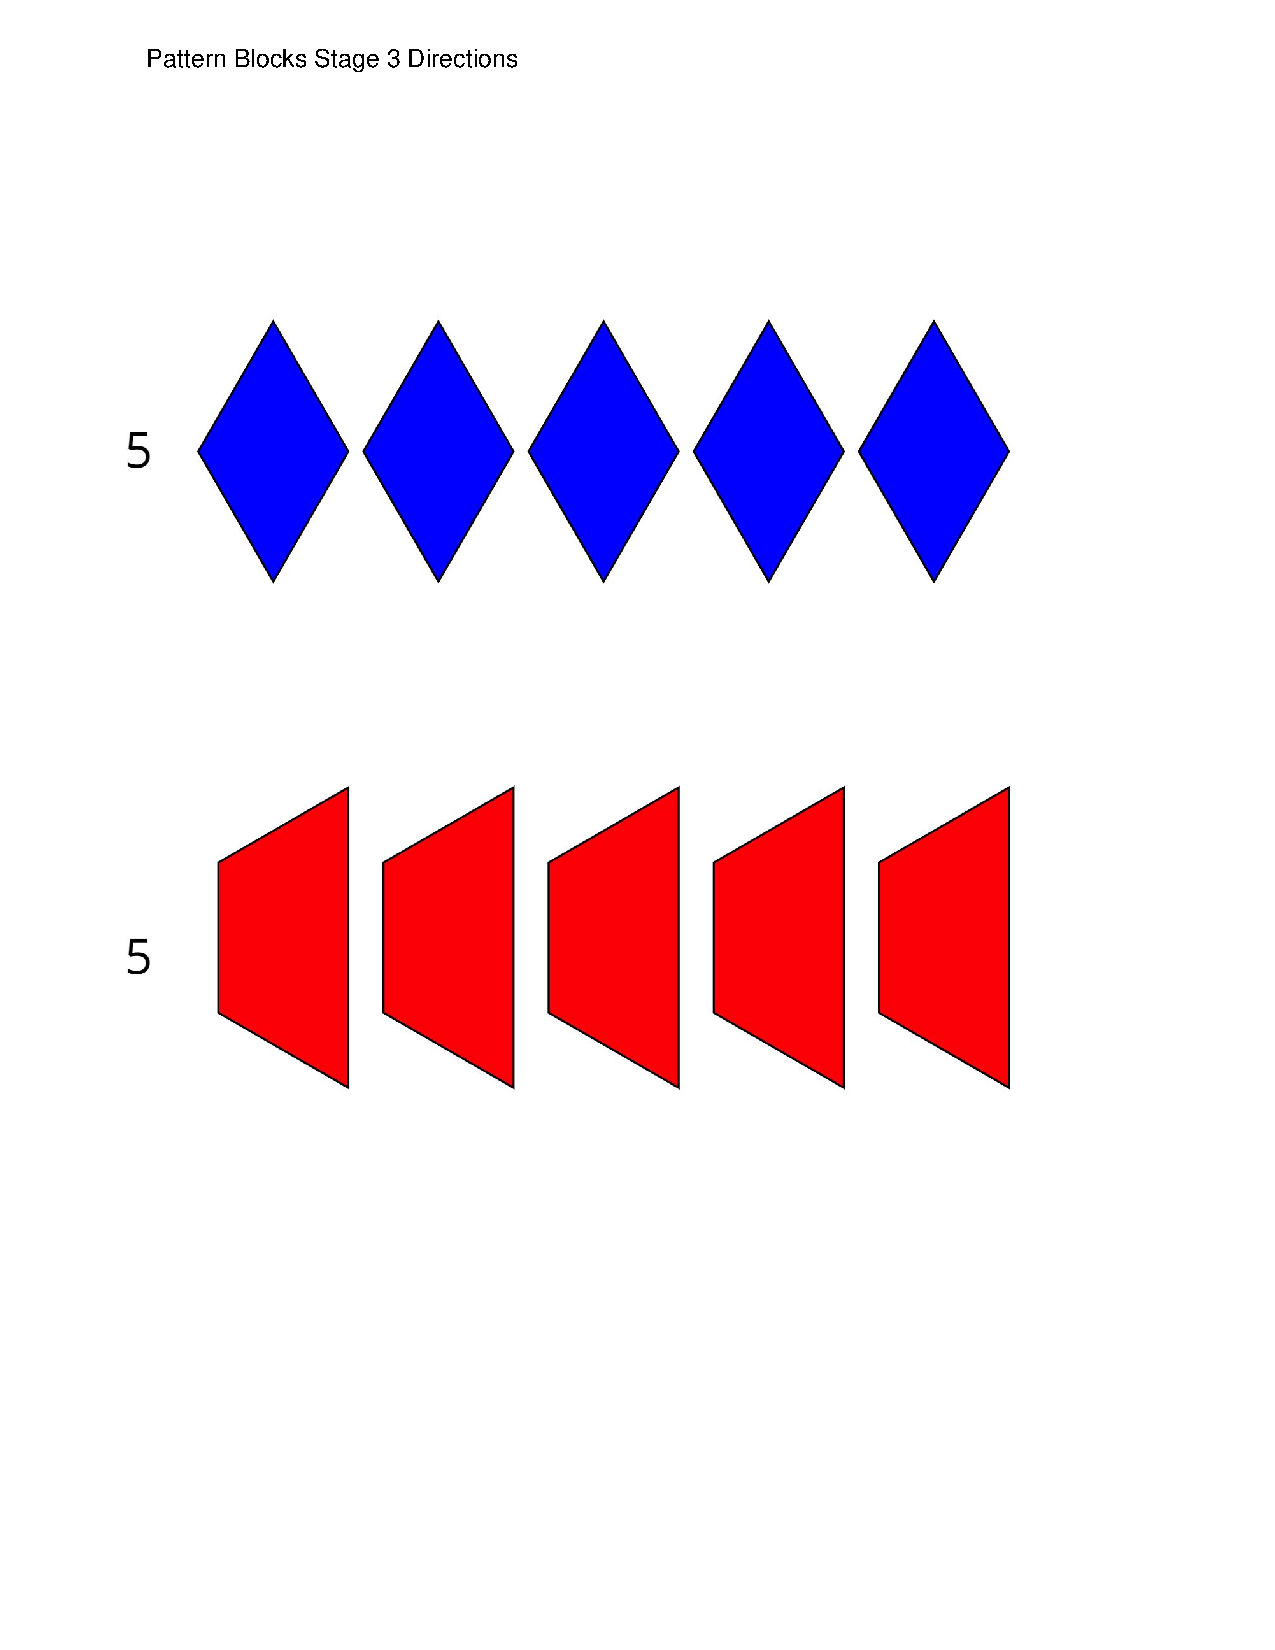
\includegraphics[page=1, trim=10 30 50 50, clip, center]{external/blm/pdf-source/centro-fichasGeometricas-etapa3.pdf}
\clearpage
\includegraphics[page=2, trim=10 30 50 50, clip, center]{external/blm/pdf-source/centro-fichasGeometricas-etapa3.pdf}
\clearpage
\includegraphics[page=3, trim=10 30 50 50, clip, center]{external/blm/pdf-source/centro-fichasGeometricas-etapa3.pdf}
\clearpage
\includegraphics[page=4, trim=10 30 50 50, clip, center]{external/blm/pdf-source/centro-fichasGeometricas-etapa3.pdf}
\clearpage
\includegraphics[page=5, trim=10 30 50 50, clip, center]{external/blm/pdf-source/centro-fichasGeometricas-etapa3.pdf}
\clearpage
\includegraphics[page=6, trim=10 30 50 50, clip, center]{external/blm/pdf-source/centro-fichasGeometricas-etapa3.pdf}
\clearpage
\includegraphics[page=7, trim=10 30 50 50, clip, center]{external/blm/pdf-source/centro-fichasGeometricas-etapa3.pdf}
\clearpage
\includegraphics[page=8, trim=10 30 50 50, clip, center]{external/blm/pdf-source/centro-fichasGeometricas-etapa3.pdf}
\clearpage
\includegraphics[page=9, trim=10 30 50 50, clip, center]{external/blm/pdf-source/centro-fichasGeometricas-etapa3.pdf}
\clearpage
\includegraphics[page=10, trim=10 30 50 50, clip, center]{external/blm/pdf-source/centro-fichasGeometricas-etapa3.pdf}
\clearpage
\end{cutoutpage}
\end{activity}%
\end{subsubsectionptx}
\end{subsectionptx}
%
%
\typeout{************************************************}
\typeout{Subsección  Lección 13 -~¿Cuántos hay? (Parte 2)}
\typeout{************************************************}
%
\begin{subsectionptx}{Subsección}{Lección 13 -~¿Cuántos hay? (Parte 2)}{}{Lección 13}{}{}{lec-cuantosHayParte2}
%
%
\typeout{************************************************}
\typeout{Subsubsección  Actividad 1}
\typeout{************************************************}
%
\begin{subsubsectionptx}{Subsubsección}{Actividad 1}{}{Actividad 1}{}{}{lec-cuantosHayParte2-act1}
\begin{activity}{Actividad}{Contemos colecciones.}{act-contemosColecciones2}%
Contemos otra colección de objetos%
\end{activity}%
\end{subsubsectionptx}
\end{subsectionptx}
%
%
\typeout{************************************************}
\typeout{Subsección  Lección 14 -~Respondamos preguntas tipo “¿Cuántos?”}
\typeout{************************************************}
%
\begin{subsectionptx}{Subsección}{Lección 14 -~Respondamos preguntas tipo “¿Cuántos?”}{}{Lección 14}{}{}{lec-preguntasTipoCuantos}
%
%
\typeout{************************************************}
\typeout{Subsubsección  Actividad 1}
\typeout{************************************************}
%
\begin{subsubsectionptx}{Subsubsección}{Actividad 1}{}{Actividad 1}{}{}{lec-preguntasTipoCuantos-act1}
\begin{activity}{Actividad}{Contemos colecciones: ¿Cuántos?}{act-contemosColecciones-cuantos}%
¿Cuántos objetos hay en tu colección?%
\end{activity}%
\end{subsubsectionptx}
%
%
\typeout{************************************************}
\typeout{Subsubsección  Actividad 2}
\typeout{************************************************}
%
\begin{subsubsectionptx}{Subsubsección}{Actividad 2}{}{Actividad 2}{}{}{lec-preguntasTipoCuantos-act2}
\begin{activity}{Actividad}{Contemos cajas de huevos.}{act-contarCajasHuevos}%
Usen la caja de huevos para descubrir cuántos objetos hay en su colección%
\begin{cutoutpage}[alternativa de caja de huevos para contar]
\includegraphics[trim=180 30 50 50, clip, center]{external/blm/pdf-source/contemos-cajasDeHuevos.pdf}
\end{cutoutpage}
\end{activity}%
\end{subsubsectionptx}
%
%
\typeout{************************************************}
\typeout{Subsubsección  Actividad 3}
\typeout{************************************************}
%
\begin{subsubsectionptx}{Subsubsección}{Actividad 3}{}{Actividad 3}{}{}{lec-preguntasTipoCuantos-act3}
\begin{activity}{Actividad}{Conozcamos “Cubos encajables: Consigue y construye”.}{act-conozcamos-cubosEncajables-consigueConstruye}%
\begin{image}{0}{1}{0}{}%
\includegraphics[max width=\linewidth, center]{external/svg-source/tikz-file-148187.pdf}
\end{image}%
\begin{image}{0}{1}{0}{}%
\includegraphics[max width=\linewidth, center]{external/svg-source/tikz-file-148188.pdf}
\end{image}%
\begin{cutoutpage}[hojas para “Cubos encajables: Consigue y construye” (laminar)]
\includegraphics[page=1, trim=30 60 30 35, clip, center]{external/blm/pdf-source/centro-cubosEncajables-consigueYConstruye.pdf}
\clearpage
\includegraphics[page=2, trim=30 60 30 35, clip, center]{external/blm/pdf-source/centro-cubosEncajables-consigueYConstruye.pdf}
\clearpage
\includegraphics[page=3, trim=30 60 30 35, clip, center]{external/blm/pdf-source/centro-cubosEncajables-consigueYConstruye.pdf}
\clearpage
\includegraphics[page=4, trim=30 60 30 35, clip, center]{external/blm/pdf-source/centro-cubosEncajables-consigueYConstruye.pdf}
\clearpage
\includegraphics[page=5, trim=30 60 30 35, clip, center]{external/blm/pdf-source/centro-cubosEncajables-consigueYConstruye.pdf}
\clearpage
\includegraphics[page=6, trim=30 60 30 35, clip, center]{external/blm/pdf-source/centro-cubosEncajables-consigueYConstruye.pdf}
\clearpage
\includegraphics[page=7, trim=30 60 30 35, clip, center]{external/blm/pdf-source/centro-cubosEncajables-consigueYConstruye.pdf}
\clearpage
\includegraphics[page=8, trim=30 60 30 35, clip, center]{external/blm/pdf-source/centro-cubosEncajables-consigueYConstruye.pdf}
\clearpage
\includegraphics[page=9, trim=30 60 30 35, clip, center]{external/blm/pdf-source/centro-cubosEncajables-consigueYConstruye.pdf}
\clearpage
\includegraphics[page=10, trim=30 60 30 35, clip, center]{external/blm/pdf-source/centro-cubosEncajables-consigueYConstruye.pdf}
\end{cutoutpage}
\end{activity}%
\end{subsubsectionptx}
\end{subsectionptx}
%
%
\typeout{************************************************}
\typeout{Subsección  Lección 15 -~Expliquemos cómo contamos}
\typeout{************************************************}
%
\begin{subsectionptx}{Subsección}{Lección 15 -~Expliquemos cómo contamos}{}{Lección 15}{}{}{lec-explicarConteo}
%
%
\typeout{************************************************}
\typeout{Subsubsección  Actividad 1}
\typeout{************************************************}
%
\begin{subsubsectionptx}{Subsubsección}{Actividad 1}{}{Actividad 1}{}{}{lec-explicarConteo-act1}
\begin{activity}{Actividad}{Contemos colecciones: Comparte cómo contaste.}{act-contemosColecciones-comparteConteo}%
¿Cuántos objetos hay en su colección?%
\end{activity}%
\end{subsubsectionptx}
%
%
\typeout{************************************************}
\typeout{Subsubsección  Actividad 2}
\typeout{************************************************}
%
\begin{subsubsectionptx}{Subsubsección}{Actividad 2}{}{Actividad 2}{}{}{lec-explicarConteo-act2}
\begin{activity}{Actividad}{Usemos un tablero de conteo para llevar la cuenta [Opcional].}{act-tableroConteoLlevarCuenta}%
Usemos un tablero de conteo.%
\end{activity}%
\end{subsubsectionptx}
\end{subsectionptx}
%
%
\typeout{************************************************}
\typeout{Subsección  Lección 16 -~Representemos nuestras colecciones}
\typeout{************************************************}
%
\begin{subsectionptx}{Subsección}{Lección 16 -~Representemos nuestras colecciones}{}{Lección 16}{}{}{lec-representarColecciones}
%
%
\typeout{************************************************}
\typeout{Subsubsección  Actividad 1}
\typeout{************************************************}
%
\begin{subsubsectionptx}{Subsubsección}{Actividad 1}{}{Actividad 1}{}{}{lec-representarColecciones-act1}
\begin{activity}{Actividad}{Contemos colecciones: Muestra cuántos.}{act-contemosColecciones-muestraCuantos}%
¿Cuántos objetos hay en su colección?%
\end{activity}%
\end{subsubsectionptx}
%
%
\typeout{************************************************}
\typeout{Subsubsección  Actividad 2}
\typeout{************************************************}
%
\begin{subsubsectionptx}{Subsubsección}{Actividad 2}{}{Actividad 2}{}{}{lec-representarColecciones-act2}
\begin{activity}{Actividad}{Respondamos preguntas tipo "¿Cuántos?".}{act-preguntasTipoCuantos}%
¿Cuántos objetos hay en su colección?%
\end{activity}%
\end{subsubsectionptx}
\end{subsectionptx}
%
%
\typeout{************************************************}
\typeout{Subsección  Lección 17 -~Esculturas con cubos encajables (opcional)}
\typeout{************************************************}
%
\begin{subsectionptx}{Subsección}{Lección 17 -~Esculturas con cubos encajables (opcional)}{}{Lección 17}{}{}{lec-esculturasCubosEncajables}
%
%
\typeout{************************************************}
\typeout{Subsubsección  Actividad 1}
\typeout{************************************************}
%
\begin{subsubsectionptx}{Subsubsección}{Actividad 1}{}{Actividad 1}{}{}{lec-esculturasCubosEncajables-act1}
\begin{activity}{Actividad}{Contemos cubos.}{act-conectemosCubosEncajables}%
¿Cuántos cubos hay en tu colección?%
\end{activity}%
\end{subsubsectionptx}
%
%
\typeout{************************************************}
\typeout{Subsubsección  Actividad 2}
\typeout{************************************************}
%
\begin{subsubsectionptx}{Subsubsección}{Actividad 2}{}{Actividad 2}{}{}{lec-esculturasCubosEncajables-act2}
\begin{activity}{Actividad}{Creaciones con cubos encajables.}{act-creacionesCubosEncajables}%
Usa todos tus cubos encajables para crear lo que quieras.%
\end{activity}%
\end{subsubsectionptx}
\end{subsectionptx}
\end{sectionptx}
%
%

%
\typeout{************************************************}
\typeout{Referencias  Atribuciones de imágenes}
\typeout{************************************************}
%
\clearpage
\begin{references-section}{Referencias}{Atribuciones de imágenes}{}{Atribuciones de imágenes}{}{}{gra0-uni1-9}
Las imágenes sin atrubición las produjo LEMA \href{https://www.grupolema.org}{www.grupolema.org}\footnote{\nolinkurl{www.grupolema.org}\label{gra0-uni1-9-2-2}} específicamente para esta adaptación y se liberan con una licencia Creative Commons Attribution 4.0 International License (CC BY 4.0), o son © 2021 \href{https://curriculum.illustrativemathematics.org}{Illustrative Mathematics}\footnote{\nolinkurl{curriculum.illustrativemathematics.org}\label{gra0-uni1-9-2-4}} con una licencia Creative Commons Attribution 4.0 International License (CC BY 4.0) y se reproducen directamente de la versión en Español disponible en \href{https://im.kendallhunt.com/K5_ES/curriculum.html}{im.kendallhunt.com}\footnote{\nolinkurl{im.kendallhunt.com/K5_ES/curriculum.html}\label{gra0-uni1-9-2-6}}.%
\end{references-section}
%
%

\end{document}
